 %!TEX root = ../main.tex
 \chapter{Improving the Robustness of Cyber-Physical System Models}
 \label{ch:CPSRobustness}  
 {\color{red}
 We now consider a practical scenario where we use spatial transformations to model both attacks and counterattacks. From the perspective of LBA, attacks and counterattacks are distinguishable only by intent: an attack is a spatial transformation that aims to damage a system, while a counterattack is a spatial transformation that tries to fix it. Recall the automaton from Section~\ref{sec:Latent:Motivation}; the spatial transformation that affected the system was a symmetry $m$ that is its own inverse (i.e., $m\circ m=\id$), so we can counter $m$ by applying it a second time. 
 
 The inclusion of counterattacks alters the interaction between attacker and system. Up until now, the LBA of a system $(X,c)$ with respect to a spatial transformation $m\colon X\rightarrow X$ that reveals the latent system $(X,c\circ m)$, which models the the system $(X,c)$ under the effect of the attack $m$. In this chapter, we consider a second spatial transformation $w\colon X\rightarrow X$ that reveals the system $(X, c\circ w\circ m)$, which models the system $(X,c)$ under the effect of the attack $m$, but also under the effect of the counterattack $w$.
 }
% In cyber-physical systems (CPSs), most security efforts aim to protect the integrity of some physical component (e.g., the level of water or chemical concentration in a tank, the temperature of an oven, etc.). The goal of integrity attackers of CPSs is to cause the system to reach a critical state by manipulating certain digital or physical inputs, e.g., by tampering with one or more sensor or actuators. The robustness of a system is a measure of tolerance to corruption introduced by external factors, be it a fault or an attacker. In this chapter, we use LBA to quantify the robustness of a CPS model via testing, and to suggest repairs which improve the robustness of the system.
   
% Using the theory of LBA, we 
% To test a system, we compose the original transition function of the CPS with the transformations induced by the attacker to obtain a new transition function that we test with respect to a set of given integrity requirements. For each successful attack (i.e., an attack that breaks one or more requirements), we use the same testing approach to find suitable counterattacks, which are dual transformations to attacks in the sense that their goal is to enforce integrity requirements. 
   
%    To test the usefulness of LBA, we apply it to a CPS model of a water treatment testbed. From the data generated by the analysis, we quantify the robustness of the testbed, and we obtain hints on how to improve the robustness of the system based on the relations between attacks and counterattacks.

% \todo[inline]{@John: Please review this introduction to CPSs (in red). We are trying to answer the question: why did you choose CPSs for this analysis and why attacks on CPS are very problematic? I guess we should make some specific emphasis on why physical components are critical and all that. Please edit as you see fit. }
%\color{blue}
\section{Introduction}
%\paragraph{Cyber-Physical Systems.} 
A \emph{cyber-physical system} (CPS) is a networked specialised computer network that monitors and controls physical components. %They vary in size and purpose. 
Some examples of CPSs include autonomous vehicles, aircraft, water treatment plants, industrial control systems, and critical infrastructures. 
A subgroup of CPS, called \emph{infrastructure} or \emph{industrial control systems} (ICS), are responsible for critical services in modern societies, such as access to clean water and transportation. Security violations in infrastructure have significant consequences in the physical world, \emph{e.g.,} in late 2007 or early 2008, the Stuxnet attack against an Iranian control system allegedly sabotaged centrifuges in uranium enrichment plants, causing them to rapidly deteriorate \cite{StuxnetWeb,Stuxnet}.
In 2014, hackers struck a steel mill in Germany and disrupted the control system, which prevented a blast furnace from properly shutting down, causing massive damage to the facility \cite{WiredArticle,Lagebericht2014}.
Other infrastructures affected by cyberattacks are a power grid in Ukraine~\cite{cherepanov2017industroyer} and oil systems in the middle-east~\cite{johnson2018attackers}.

% \todo[inline]{@All: sections in blue seem secondary and could be removed. Do you object? The intro is way too long as it is...}
{
%\color{blue}

% Although \emph{confidentiality} has traditionally enjoyed more attention than \emph{integrity} in the scientific literature on information security, we must protect integrity as observed for instance by Clark and Wilson \cite{ClarkWilson87}: ``in the commercial environment, preventing disclosure is often important, but preventing unauthorized data modification is usually paramount.''
{%\paragraph{Integrity in CPSs.} 
Protecting the integrity of CPSs is paramount. This is especially true for ICSs; their security priority is not the protection of confidential data, but the protection of their physical assets. Gollmann and Krotofil reinforce this view in \cite{CPSSec}, stating that the traditional CIA (Confidentiality-Integrity-Availability) triad should be reversed when studying the security of CPSs. They argue that the enforcement of integrity in CPSs should not only consider the ``traditional approach for IT systems'', {i.e.}, protecting {component logic} and {communication}, but that we must also protect the integrity of {observations}; more precisely, we have to protect the {veracity} of sensor data and check its {plausibility}.} 

A \emph{robust} CPS can tolerate the presence of external perturbations (i.e., attacks or faults). In other words, the integrity of the system is preserved in the presence of adversaries. Traditionally, the enforcement of CPS integrity has  used {control-theoretic methodologies}, specifically {fault-detection techniques}. Control theory researchers model attacks on CPSs as time-series with specific structures affecting sensor measurements and/or control commands. Depending on their capabilities, attackers have the power to control when, where, and how attacks enter the system. Research on attack detection and mitigation has mainly focused on the so-called \emph{integrity attacks}, i.e., attacks that put at risk the proper operation and physical integrity of CPSs. Integrity attacks include stealthy attacks \cite{CPSStealthAttacks}, message replay \cite{CPSReplayAttacks}, covert attacks \cite{CPSCovertAttacks}, and false-data injection \cite{CPSDataInjectionAttacks}, among others. Due to their focus on fault-detection techniques, many results based on control theory aim to protect CPSs from integrity attacks in two ways: one, by first verifying that their system satisfies a series of security guarantees during {normal operation} (i.e., attack-free operation), and second, by relying on {monitoring} the physics of the system to detect anomalies (see, e.g., \cite{CPSInvariantsForDetection,Urbina2016,CPSAttackDetection,CPSAttacksAgainstPCS,CPSIntegrityAttacks,CPSDetectingIntegrityAttacksScada}). 

From the computer science perspective, we can estimate the robustness of software systems by systematic \emph{fault injection} through techniques like fuzzing (see~\cite{Fuzzing}).  
%\todo[inline]{@All: do you know of relevant fault injection papers that we can cite here? I'm familiar with only a couple, and mostly related to fuzzing and mutation testing}
During fault injection, we provide semi-random inputs to the system in the hopes of creating new behavioural traces that may be insecure.  % The notion of robustness may slightly vary from the degree of a system to tolerate deviations from its normal behaviour~\cite{}
% \todo[inline]{@John: can you please explain and cite a definition of Robustness for CPSs? }
% \todo[inline]{@All: we are still missing this bit in blue about an accepted definition of robustness... we'll update it ASAP.}
Normally, an insecure systems is a system with abnormal termination, but we can extend this notion to other security properties if we have a decision procedure to determine when an input is successful at breaking the security properties. In our CPS scenario, the inputs that we use to quantify robustness are the attacks that correspond to some given attacker model. We also assume the existence of a set of security requirements $\TheSetOfRequirements$ that we can evaluate in the CPS. Henceforth, we consider a CPS to be robust with respect to a set of attacks $\mathcal{M}$ and a set of requirements $\TheSetOfRequirements$ if no attack in $\mathcal{M}$ can break any security requirement in $\TheSetOfRequirements$. 

Following the LBA methodology, we model attacks as spatial transformations, and we compose these transformations with the original system to create a latent system. We test the latent systems to quantify the robustness of the original system: if a latent system fails a security requirement, then the CPS is vulnerable to the attack that reveals the latent system. Similar to the control theoretical approaches, we expect that the system under normal circumstances satisfies all the security requirements in $\TheSetOfRequirements$. However, it is not unexpected that the system fails to satisfy one or more security requirement while it is under attack. 

To protect the CPS in scenarios that are not attack free, we propose the use of \emph{counterattacks}. A counterattack is a second spatial transformation that aims to counter the effect of one or more attacks. More precisely, if we model a CPS whose set of states is $\Pi$ and whose transition function is $\TheSystem\colon\Pi\rightarrow\Pi$, we can compose $\TheSystem$ with a state transformation $m\colon \Pi\rightarrow\Pi$ that models an attack and reveal a the latent CPS $(\Pi,m\circ \TheSystem)$. To counter $m$, we introduce a second spatial transformation $w\colon \Pi\rightarrow \Pi$ to reveal a latent CPS $\TheSystem\circ w\circ m$ that satisfies the following property: if the system $(\Pi,\TheSystem\circ w\circ m)$ satisfies all security requirements that the original CPS does, then $w$ counters the attack $m$.

%latent transition function $\TheSystem\circ m\colon\Pi\rightarrow\Pi$. The original system is modelled by a tuple $(\Pi,\TheSystem)$, and the tuple $(\Pi,\TheSystem\circ m)$ models the system when it is under the attack $m$. 
% If the system $(\Pi,\TheSystem\circ m)$ fails a security requirement, then the system $(\Pi,\TheSystem)$ is vulnerable to the attack $m$. 
% To avoid relying on monitors, we use a testing-based approach that simulates the system in the presence of attacks. %,
}
%\todo[inline]{@ALL: let me try to sell the latent behaviour analysis method to you. If you think this following argument is weak, please let me know. }

% For example, in the context of fault injection, a fault $m$ that flips a bit of a registry, transforms the current state of the registry, but leaves the transition function $\delta$, i.e., the rules to compute the next state of the registry, intact. Nevertheless, the composition of the spatial transformation $m$ and the transition function $\delta$ create a new transition function $\delta\circ m$, which characterises a new transition system. LBA studies the behavioural properties of the $\delta\circ m$ transition system, 
%We use spatial transformations to stress the system so it fails its security requirements. However, we can turn the roles around, and try to find a set of ``counter-faults'' which invalidate $m$. We can then give the set of counter faults to the designer so that they can use them as a starting point for redesigning reaction mechanisms for when an attack is detected. 

Theoretically, for a system $(\Pi,\TheSystem)$, %if the set of states $\Pi$ is finite, there are $|\Pi|^{|\Pi|}$ 
it is possible to arbitrarily choose values for the spatial transformations $m$ (attack) and $w$ (counterattack) from the set of endofunctions $\Pi^{\Pi}$.  However, in the case of $m$, this set of transformations models an attacker that is capable of arbitrarily morphing the state of the CPS, including both cyber and physical aspects, in any form and at any time. This attacker is trivially too powerful to defend against, not to mention impossible, since it would be capable of bypassing physical invariants (e.g. Boyle's law). To model realistic attackers, we use attacker models that are a combination of simple actions that affect individual components (e.g., set a fixed value in a sensor). Now, since attacks and counterattacks are duals, we model realistic counterattackers by using a combination of simple actions that affect individual variables in the controllers of the CPS. We also illustrate how, based on the interactions between attacks and counterattacks, the designers of CPSs can derive possible repairs for the CPS such that the robustness of the system provably increases.

%  We use the new transition function $\TheSystem\circ m$ to quantify the robustness of the original system in the same spirit as fault injection. Then, because attacks and counterattacks are duals of the same type, we define a counterattacker model to try to find, for each attack $m\colon\Pi\rightarrow\Pi$, a counterattack $w\colon\Pi\rightarrow\Pi$. We also show how attack-counterattack pairs can give the designer of the CPS useful insights on how to make the control strategy provably more robust. % and how to implement mitigation mechanisms that are more effective.

% Formally, any transformation $m\colon\Pi\rightarrow\Pi$ can be used to reveal a latent behaviour. 
% However, we are interested in those $m$ that model realistic attacks. 
% In this work, we provide a framework to define attacks and attackers, and a method to systematically generate them, yielding a universe $\mathcal{A}$ of attackers and a universe $\mathcal{M}$ of attacks.
% , and two mappings between them: 
% the mapping $\texttt{has}\colon\mathcal{A}\rightarrow\mathscr{P}(\mathcal{M})$ which maps each attacker to the set of attacks they can perform, and a mapping $\texttt{minimal}\colon\mathcal{M}\rightarrow \mathcal{A}$, which maps each attack to the attacker with minimal capabilities that can perform it.

% \todo[inline]{@Eric: explain what it means for a system to be robust and how to quantify its robustness.}
% \todo[inline]{Here is where i'm a bit stuck and why it is important to do some experiments. I'm working together with John and Sudipta to define interesting use cases for our Latent behaviour analysis (LBA)}
%Instead of determining whether a system is secure or not, we are interested in the following decision problem: given two candidate designs of system, decide which one is more secure.% and determining what aspects of the system require more urgent redesign. 
%  the set $\texttt{Vulnerabilities}\subseteq $, of attacks that can break a security requirement, and a metric for attackers, named $\texttt{flexibility}\colon \mathcal{A}\rightarrow \mathscr{P}(\mathcal{M})$ which maps each attacker to the set of their successful attacks (i.e. attacks that can break at least one security requirement). 

% In this work, we measure the security of the system by counting the number of attacks that are successful.

%%%%%%%%%%%%%%%%%%%%%%%%%%%%%%%%%%%%%%%%%%
%          Chemical toy example
%\input{old_sections/old_Introduction} 
%%%%%%%%%%%%%%%%%%%%%%%%%%%%%%%%%%%%%%%%%%

\textbf{Problem statement:} To summarize, in this work we address the following
questions: how can we systematically generate realistic attacks and counterattacks for a CPS model? %\emph{Can we identify at design time which inputs to a CPS are most
%harmful if controlled by an attacker? 
How can we improve the design of the CPS at design time and justify our models formally with respect to a quantitative notion of robustness?

\textbf{Summary of our Approach:} We propose to model a CPS as a composition of the control logic and the physical system in terms of a deterministic transition system. We then formally quantify the impact of various attackers using the following testing approach: using LBA, we obtain a family of systems that model the CPS in the presence of attackers and counterattackers, which we test via simulation to identify successful attacks and counterattacks. We quantify the robustness of the system by counting the number of successful attacks, and we quantify a potential for improvement by counting the number of successful attacks that can be countered by at least one counterattack. We note that a sound implementation of the counterattacks requires the existence of an attack monitor that has strong precision and correctness requirements, so, alternatively, by observing the interactions between attacks and counterattacks, we propose a repair, i.e., a modification of the program of the controller of the CPS. To assess the success of the repair, we compare the robustness of the repaired version to the robustness of the original system; if the robustness of the repaired system is strictly higher than the robustness of the original, then the repair is successful. 

\textbf{Contributions:} We make the following contributions \textbf{a)} We present a logical framework to formally reason about robustness in CPS models using spatial transformations, 
reconciling testing techniques and control theoretical aspects. \textbf{b)} We discuss how our approach can be used to model attacks, counterattacks, and quantify the robustness of CPSs. \textbf{c)} We illustrate the usefulness of
our approach by means of simple but realistic models concerning a water
distribution CPS; we show that we can identify non-trivial attacks and counterattacks, and we show how to implement a repair that provably improves the robustness of the original system.

{
\section{Control Theory Preliminaries}
% \todo[inline]{Do we really need to present control theory preliminaries? Or is there an IT approach to CPS attacks?}
Gollmann and Krotofil highlight, ``to work on cyber-physical systems, one has to combine the devious mind of the security expert with the technical expertise of the control engineer''~\cite{CPSSec}. 
Unfortunately, this expertise is ``not commonly found in the IT security community''~\cite{CPSSecVinyl}. 
% according to the authors of  
Moreover, the language barrier between control theory and IT security disciplines worsens this lack of expertise.
Thus, in this section, we present the model-based techniques for CPSs security broadly used by the systems and control community.
\subsection{Linear Time-Invariant Models.} 
During the last decade, there has been an increasing tendency to use physics-based models of CPSs to detect and quantify the effect of attacks on the system performance \cite{CPSAttacksAgainstPCS,Urbina2016,CPSDetectingIntegrityAttacksScada,CPSIntegrityAttacks,Carlos_Justin1,Carlos_Justin2,ReachableSets}. These physics-based models focus on the normal operation of the CPS and work as prediction models that are used to confirm that control commands and measurements are valid and plausible. Often, dynamical models of physical systems are approximated around their operation points or approximated using input-output data. These lead to approximated models which are often linear and time-invariant.

Following the work in \cite{CPSAttacksAgainstPCS,Urbina2016,CPSDetectingIntegrityAttacksScada,CPSIntegrityAttacks,Carlos_Justin1,Carlos_Justin2,ReachableSets}, here, we only consider Linear-Time Invariant (LTI) models, although the same ideas are employed when considering more complicated dynamics. In particular, a model of a CPS that uses LTI stochastic difference equations is of the form
\begin{equation}
\left\{
\begin{array}{ll}
{x}({k+1}) = Ax(k) + B u(k) + \vartheta(k),  \label{1} \\[1mm]
\hspace{3.8mm} y(k) = Cx(k) + \eta(k),
\end{array}
\right.
\end{equation}
with $k\in \Nat$, physical state of the system $x \in \Real^n$ (i.e., an $n$-dimensional vector of physical variables associated with the dynamics of the CPS), sensor measurements $y := (y_1,\ldots,y_m)^T \in \Real^m$ , control commands $u := (u_1,\ldots,u_m)^T \in \Real^l$, real-valued matrices $A$, $B$, and $C$ of appropriate dimensions, and i.i.d. multivariate zero-mean Gaussian noises $\vartheta \in \Real^n$ and $\eta \in \Real^m$ with covariance matrices $R_{1} \in \Real^{n \times n}$ and $R_2 \in \Real^{m \times m}$, respectively. The matrix $A$ describes the \emph{dynamic evolution of the physical process}, $B$ is used to model the effect of \emph{actuators} on the system dynamics, and the matrix $C$ models the part of the state $x_k$ available from \emph{sensor measurements}.

\subsection{Attacks on Models of CPSs}
\label{sec:CPSRobustness:AttacksOnModels} 
At the time-instants $k \in \Nat$, the output of the process $y(k)$ is sampled and transmitted over a communication network. The received output is used to compute control actions $u(k)$ which are sent back to the physical process. The complete control-loop is assumed to be performed instantaneously, i.e., the sampling, transmission, and arrival time-instants are supposed to be equal.
In between transmission and reception of sensor data and control commands, an attacker may replace the values coming from the sensors to the controller and from the controller to the actuators, acting as a {man-in-the-middle}. Thus, after each transmission and reception, the attacked output $\bar{y}$ and attacked input $\bar{u}$ take the form
\begin{equation}
\left\{
\begin{array}{ll}
\bar{y}(k) := y(k) + \delta^y(k) 
, \label{3}\\[1mm]
\bar{u}(k) := u(k) + \delta^u(k),
\end{array}\right.
\end{equation}
where $\delta^y(k) \in \Real^m$ and $\delta^u(k) \in \Real^l$ denote \emph{additive sensor and actuator attacks}, respectively.

%Henceforth, we denote $x(k)$ by $x_k$, $ \bar{u}(k)$ by $\bar{u}_k$, $\vartheta(k)$ by $\vartheta_k$, $\bar{y}(k)$ by $\bar{y}_k$, $\eta(k)$ by $\eta_k$, $\delta^y(k)$ by $\delta_k^y$, and $\delta^u(k)$ by $\delta^u_k$. Then, a
A system under attack is modelled by
\begin{equation}
% \left\{
% \begin{array}{ll}
% {x}_{k+1} = A x_k + B (u_k + \delta^u_k) + \vartheta_k,\label{17} \\
% \text{ \ \ }\hspace{.35mm}\bar{y}_k = C x_k + \eta_k + \delta^y_k.
% \end{array}
% \right.
\left\{
\begin{array}{ll}
{x}({k+1}) = A x(k) + B (u(k) + \delta^u(k)) + \vartheta(k),\label{17} \\
\text{ \ \ }\hspace{.35mm}{y}(k) = C x(k) + \eta(k) + \delta^y(k).
\end{array}
\right.
\end{equation}
}
\section{Motivational Example: A Water Tank}
\label{sec:CPSRobustness:example}
We now provide a simple example to motivate the problem of quantifying robustness via testing in CPS models. We also illustrate the concepts behind the modelling formalisms presented in the following sections, especially LBA.
%==================BEGIN JOHN WORKSPACE====================

%==================END JOHN WORKSPACE====================

% In this section, we model SWaT's the water tank process as a LTI system, and we describe attackers for it in the traditional sense (i.e. attackers on its sensors and actuators)...
%\begin{wrapfigure}{tr}{0.5\textwidth}
\begin{figure}
  \centering
  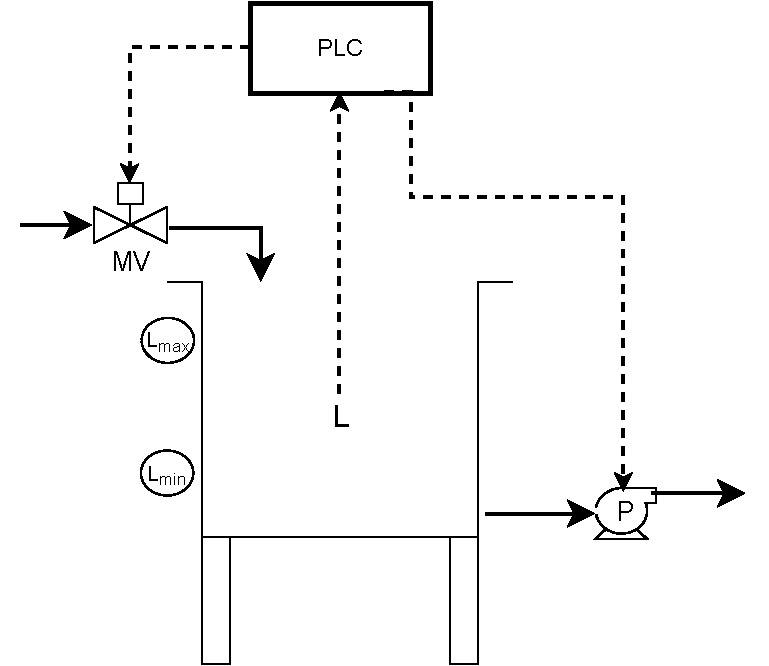
\includegraphics[width=0.50\textwidth]{Figures/FillingTank.pdf}
  \caption{A water tank. The PLC sends control commands to the motor valve (MV) and the pump (P) so that the level of the tank (L) stays within the range $L_{min}$ -- $L_{max}$. }
  \label{fig:CPSRobustness:Motivational}
%\end{wrapfigure}
\end{figure}
%To quantify the robustness of a CPS, we first need to define its model. 
Consider the following model of a CPS containing a water tank with a water level (L), a water pump (P), a motor valve (MV), and a programming logic controller (PLC), as shown in Figure~\ref{fig:CPSRobustness:Motivational}. This system has a physical process state vector $\vec{x}$, a cyber controller state vector $\vec{q}$, a sensor state vector $\vec{y}$, and an actuator state vector $\vec{u}$.

The physical state vector $\vec{x}$ has coordinates $MV$, $L$ and $P$, where $\vec{x}[MV]$ corresponds to the physical state of the motor valve, $\vec{x}[P]$ corresponds to the physical state of the pump, and $\vec{x}[L]$  corresponds to the physical state of the water level of the tank. The variable $\vec{x}[MV]$ can take four values: $\texttt{closed}$, $\texttt{opening}$, $\texttt{open},$ or $\texttt{closing}$. The variable $\vec{x}[P]$ can take two values: $\texttt{on}$ and $\texttt{off}$. Finally, the variable $\vec{x}[L]$ can take any value between $0 ~\mathrm{L}$ and $1200 ~\mathrm{L}$ (the maximum capacity of the tank). %\begin{figure}[t]
%\begin{wrapfigure}[lineheight]{position}{width}
%\end{figure}
Depending on the state of the motor valve $\vec{x}[MV]$, different amounts of water flow into the tank. In turn, the state of the valve $\vec{x}[MV]$ changes when it receives the control input $\vec{u}[MV]$, which can take the values $\texttt{closed}, \texttt{opening},\texttt{open},$ or $\texttt{closing}$.  

The behaviour of the physical process is captured by the following linear time invariant system:
\begin{align}
  \vec{x}[L](k+1)&= \vec{x}[L](k)+Inflow(k)-Outflow(k),\quad \text{where}\\
  Inflow(k)&=\begin{cases}
    0.31,&\quad \text{if $\vec{x}[MV](k)=\texttt{open}$}\\
    0,&\quad \text{if $\vec{x}[MV](k)=\texttt{closed}$}\\
    0.26,&\quad \text{otherwise}\\
  \end{cases}\\
  Outflow(k)&=\begin{cases}
    0.15,&\quad \text{if $\vec{x}[P](k)=\texttt{on}$}\\
    0,&\quad \text{otherwise}\\
  \end{cases}\\
    % \begin{cases}
    %   \vec{x}[L](k)+0.16,&\quad \text{if $(\vec{x}[MV](k),\vec{x}[P](k))=(\texttt{open}$,\texttt{on})}\\
    %   \vec{x}[L](k)-0.15,&\quad \text{if $\vec{x}[MV](k)=\texttt{closed}$,}\\
    %   \vec{x}[L](k)+0.11,&\quad \text{otherwise;}\\
    % \end{cases}\\
  \vec{x}[MV](k+1)&=\vec{u}[MV](k)\\
  \vec{x}[P](k+1)&=\vec{u}[P](k)\\
  \vec{y}[L](k)&=\vec{x}[L](k)
\end{align}
The value of $\vec{y}[L]$ is a measurement of $\vec{x}[L]$, but since it is a cyber component, it can take values above 1200 (although in normal circumstances it remains in the range $[0..1200]$). We leave the initial conditions of the process abstract for now.

The values of the control command for the motor valve $\vec{u}[MV]$ are defined by the controller, which uses $\vec{y}[L]$ to make decisions. The controller itself has a state $\vec{q}$ that has four coordinates: the presumed state the valve $MV$, denoted by $\vec{q}[MV]$, the presumed state of the pump $P$, denoted by $\vec{q}[P]$, the presumed water level of the tank $L$, denoted by $\vec{q}[L]$,  and a timer $\tau$ that the controller uses to approximate the time it takes for the motor valve $MV$ to open or close, denoted $\vec{q}[\tau]$. %These state of the valve, pump and water tank are presumed, because the controller cannot directly observe them

The controller updates its state using $\vec{y}[L]$, and produces the control values $\vec{u}[MV]$ and $\vec{u}[P]$ using $\vec{q}(k)$, with 
\begin{align}
  \label{eq:ControllerStage3}
  \vec{q}[MV](k+1)&=
  \begin{cases}
    \texttt{opening},&\quad \text{if $\vec{q}[MV](k)=\texttt{closed}$ and $\vec{y}[L](k)\leq L_{min}$,}\\
    \texttt{open},&\quad \text{if $\vec{q}[MV](k)=\texttt{opening}$ and $\vec{q}[\tau](k)>T$,}\\
    \texttt{closing},&\quad \text{if $\vec{q}[MV](k)=\texttt{open}$ and $\vec{y}[L](k)\geq L_{max}$,}\\
    \texttt{closed},&\quad \text{if $\vec{q}[MV](k)=\texttt{closing}$ and $\vec{q}[\tau_3](k) >T_3$,}\\
    MV&\quad \text{otherwise;}    
  \end{cases}\\
  \vec{q}[\tau](k+1)&=
\begin{cases}
  1+\vec{q}[\tau](k), &\quad \text{if $\vec{q}[MV](k)=\texttt{opening}$ or $\vec{q}[MV](k)=\texttt{closing}$}\\
  0,&\quad \text{otherwise;}    
\end{cases}\\
\vec{q}[L](k+1)&=\vec{y}[L](k)\\
\vec{q}[P](k+1)&=\texttt{on}\\
\vec{u}[MV](k+1)&=\vec{q}[MV](k+1)\\
\vec{u}[P](k+1)&=\vec{q}[P](k+1)
\end{align}
where $L_{min}=800$, $L_{max}=1000$ and $T=7$. We leave the initial conditions of $\vec{q}$ and $\vec{u}$ abstract for now.

Now that we have a description of the model of the CPS, we define a set of security requirements that determine whether the behaviour of the system is safe or not.

%\subsection{Security Requirements and Additive Attacks}
\subsection*{Security Requirements}
%\begin{wrapfigure}{r}{0.4\textwidth} 
 % \vspace{-1cm}
 \begin{figure}
  \centering
  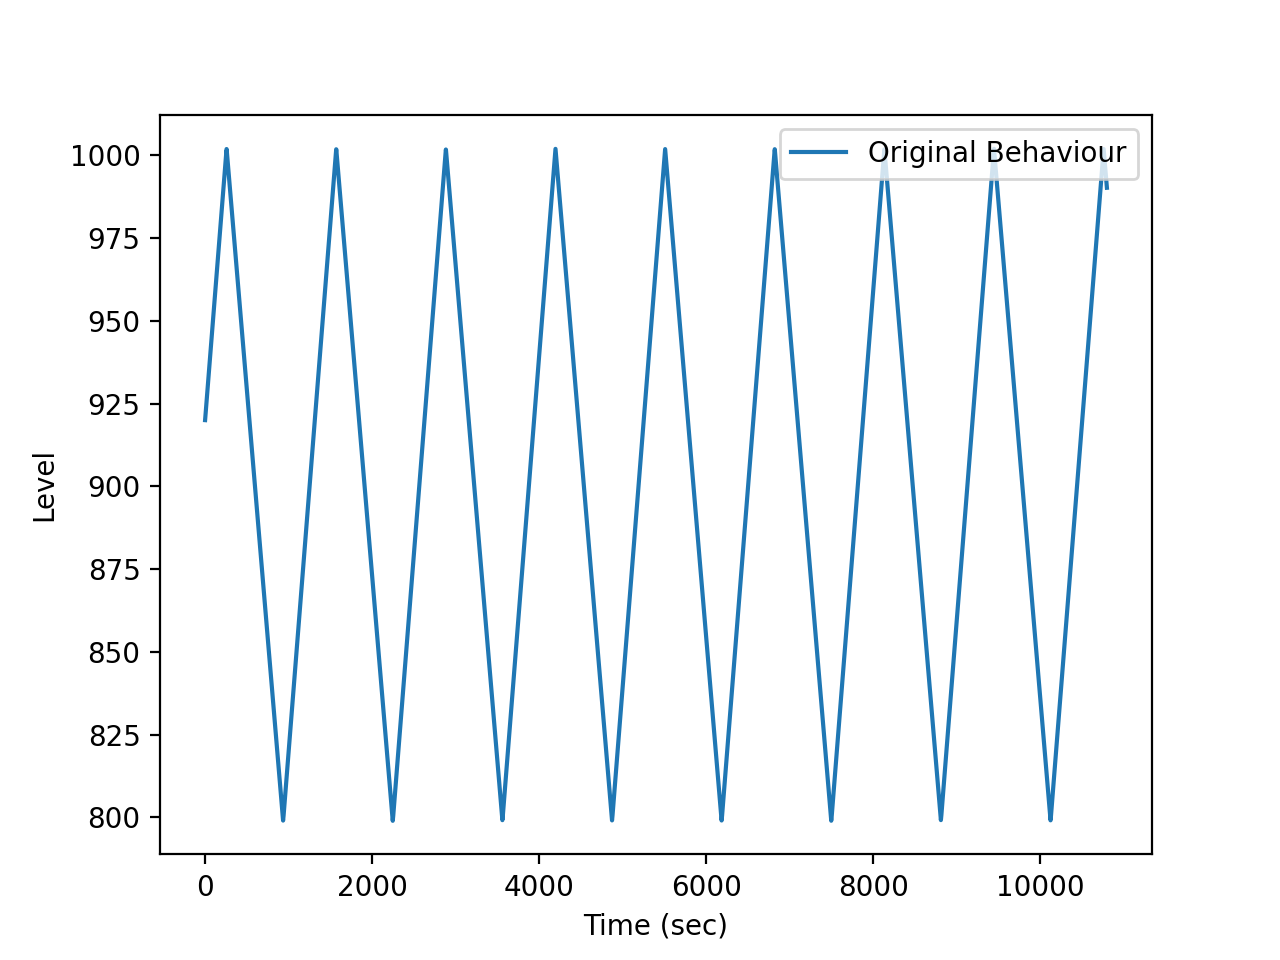
\includegraphics[width=0.5\textwidth]{Figures/Stage3Normal.png}
  %\vspace{-0.25cm}
  \caption{Normal steady state behaviour of the water level of the water tank.}
  \label{fig:CPSRobustness:Stage3Normal}
%   \vspace{-1cm}
% \end{wrapfigure} 
 \end{figure}
We establish two simple security requirements for the water tank: the tank is never empty and the tank never overflows. These requirements protect the integrity of the system: if the tank empties, the pump suffers physical damage due to cavitation, and if the tank overflows, then water spills out, causing a work hazard. Formally, these requirements correspond to the invariants $\Always{\vec{x}[L]< 1200}$ and $\Always{\vec{x}[L]> 0}$, defined by
  \begin{align*}
    \Always{\vec{x}[L]< 1200}&\triangleq \forall k\geq0.\vec{x}[L](k)< 1200,\\
    \Always{\vec{x}[L]> 0}&\triangleq \forall k\geq0.\vec{x}[L](k)> 0.
  \end{align*}
Under normal circumstances, the water level of the tank exhibits the behaviour displayed in Figure~\ref{fig:CPSRobustness:Stage3Normal}. The system in its attack-free state satisfies the security requirements $\Always{\vec{x}[L]< 1200}$ and $\Always{\vec{x}[L]> 0}$.
%\begin{figure}[t]
\subsection*{Testing and Quantifying Robustness}
Now, consider an attacker model where the attacker can replace at any time the value $\vec{y}[L]$ by a value of their choice, or use the real value. This attacker model generates a universe of 64 different \emph{representative classes of attacks}, which define when and what values to use to replace $\vec{y}[L]$. These 64 attacks classes correspond to the paths that the attacker can trigger in the controller by varying the values of $\vec{y}[L]$.  More precisely, the attacker has four options: they can introduce a fake low level value (e.g., 500 L), a fake ok level value (e.g. 800 L), a fake high level value (e.g., 1100 L) or preserve the real water level value. The attacker can choose to use different actions in three main scenarios: when the water level is high, normal, or low. This combination of four ``what" values over three ``when" dimensions defines $4^3=64$ combinations. We explain in detail the generation of attack universes in Section~\ref{sec:CPSRobustness:AttackerCapabilities}. 

We measure the robustness of the system with respect to this attacker model by computing the number of attacks that do not break any of the security requirements. To test an attack in the system, we simulate several operation hours of the system while concurrently simulating the effect of the attack until either the simulation timeouts or the system fails a requirement. After testing, we see that 30 out of 64 attacks break at least one requirement, so the robustness of this system is 34/64 with respect to an attacker that has control of $\vec{y}[L]$. We explain the process of computing robustness in detail in Section~\ref{sec:CPSRobustness:LatentBehaviours}.

\subsection*{Counterattackers}
%So far, we have used a method similar to simulation-based fault-injection to quantify the robustness of the water tank with respect to an attacker that controls the sensor $\vec{y}[L]$; now, 
We now rely on the fundamental observation that an attack $m$ on the original version of the tank reveals a latent system, which we denote $T_m$, and that a transformation $w$ on the latent system $T_m$ reveals another latent system $T^w_m$, which hopefully satisfies all security requirements. In such a case, we say that \emph{$w$ is a counterattack of $m$}. 

A \emph{counterattacker model} is dual to an attacker model. It also requires a ``what" and a ``when" to act. In this scenario, we assume that the counterattacker directly changes the physical state of the pump and the valve, i.e., an operator implements this counterattacker, and they can manually set the coordinate $\vec{x}[P]$ to \texttt{on} or \texttt{off} and the coordinate $\vec{x}[MV]$ to \texttt{open} or \texttt{close}, overriding the commands of the controller. We also assume that the counterattacker can observe the value $\vec{y}[L]$ (which is controlled by the attacker in this scenario). From this counterattacker model, we generate a universe of 729 counterattacks (we explain how we obtain the size of the counterattack universe in Section~\ref{sec:CPSRobustness:CounterAttacks}).  

All 40 successful attacks can be countered, i.e., for each attack $m$ there exists a counterattack $w$ such that the system $T^w_m$ satisfies all the security requirements. Consequently, we say that the system has a \emph{latent robustness} of 64/64; i.e., it is theoretically possible for a counterattacker fitting the counterattacker model to counter every attack of an attacker fitting the attacker model, given that it is possible for the counterattacker to accurately identify that: 1) the system is under attack, and 2) which exact attack is occurring, since apparently similar attacks could have different counterattacks. Assuming the existence of such monitor is impractical; which is why we instead consider a modification of the program of the PLC based on the information that we obtain from the LBA to improve the robustness of the system. In Section ~\ref{sec:CPSRobustness:CaseStudy}, we perform LBA on a system that is more complex than the water tank, and we show how to use the relations between attacks and counterattacks obtained via LBA to propose repairs that improve the robustness of the model.  

\section{Cyber-Physical Systems, Physical Requirements and \\Attacker Models}
% Our main objective is to define a flexible testing method to determine how well the integrity of the process of a CPS is preserved in the presence of attackers. For this purpose, we now define formal notions of \emph{CPS state}, \emph{single-cycle semantics}, and \emph{physical integrity requirements}.
%\todo[inline]{Small intro that explains what this section is}
%Traditional IT security mechanisms such as authentication and message integrity are insufficient for CPS security. %However, as stated in \cite{CPSAttacksAgainstPCS}, 
The major difference between CPSs and IT systems is the interaction with the physical world. We share the view of Gollmann \emph{et al.} \cite{CPSSecVinyl}, who state that CPSs security is {specifically} concerned with attacks that cause some physical impact; i.e., attack that affect the integrity of the physical process beyond repair. The robustness of a system is a measure of tolerability to those attacks that target integrity. 
%Traditional IT security mechanisms (e.g., firewalls, encryption, signatures, etc.) normally do not account for physical parts of the system, making them ineffective when faced against attacks that either target or interact with the physical components of CPSs. In this section, we present an Information Flow (IF) inspired integrity analysis for CPSs which accounts for the physical process.

In this section, we present a framework to quantify the robustness of CPSs. This framework consists of several parts:
\begin{enumerate}
  \item a discrete model for CPSs and their semantics; 
  \item a description of physical security requirements;
  \item a formalisation of attacker models and attacks for our CPS models;
  \item a formulation of counterattacker models and counterattacks, dual to those of attackers and attacks;
  \item a quantitative notion of robustness and latent robustness based on physical security requirements, attacker models and counterattacker models.
\end{enumerate}

\subsection{A Discrete Model for CPSs}
Figure \ref{fig:CPSRobustness:IFCPS} presents an extended version of the \emph{supervisor model} \cite{doi:10.1137/0325013}, which serves as the starting point for our modelling framework. 
\begin{figure}
\centering
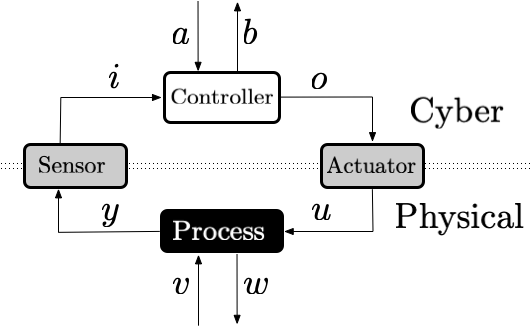
\includegraphics[width=0.45\textwidth]{Figures/IFCPS}
\caption{Extended supervisor model accounting for external inputs and outputs in both cyber and physical components.}
\label{fig:CPSRobustness:IFCPS}
\end{figure}
Our CPS model consists of four subsystems: the \emph{controller}, an open, discrete cyber system; the \emph{process}, a linear-time invariant physical system; and two sets of cyber-and-physical interface systems: the \emph{sensors} and the \emph{actuators}. The vector $\vec{q}$ models the current state of the controller, and $\vec{x}$ models the current state of the process. The vector $\vec{i}$ models cyber input measurements and the vector $\vec{o}$ models cyber control outputs; they respectively model the internal communication channels between controller and sensors, and between controller and actuators. Similarly, the vector $\vec{u}$ models the physical control inputs and the vector $\vec{y}$ models physical measurements; these vectors respectively model the internal communication channels between the process and actuators, and between the process and sensors. 

The cyber network input $\vec{a}$ and the cyber network output $\vec{b}$ enable communication between controllers, and enable CPS composition on the cyber side. Similarly, the physical network input $\vec{v}$, and the physical network output $\vec{w}$ model physical channels that connect modules of a larger physical system, enabling the composition of CPS on the physical side. For example, when two water tanks $T_1$ and $T_2$ are connected by a pipe, the outgoing flow from $T_1$ to $T_2$ (a component of $\vec{w}$ for $T_1$) should translate into the incoming flow from $T_1$ to $T_2$ (a component of $\vec{v}$ for $T_2$). 

\begin{definition}[States of a CPS]
\label{def:CPSRobustness:States}
A \emph{state of a CPS} $\pi$ is the coupling of the components of such CPS; formally, 
\begin{align}
\pi=(\vec{a},\vec{b},\vec{i},\vec{o},\vec{u},\vec{y},\vec{v},\vec{w},\vec{q},\vec{x}).
\end{align}
%$(\vec{a},\vec{b})$ is the state of the network, $(\vec{i},\vec{o},\vec{u},\vec{y})$ is the state of the channels, $(q,x)$ is the \emph{hidden} state of the controller and the process. 
%\todo[inline]{@All: for this paper this notation is fine because we do not write things like $\pi[\vec{x}[smt[smt2[smt3]]]]$ or $\pi[\vec{x}][smt][smt2]...$ which is horrible, we write $\pi[\vec{x}[L]]$,though.}
Let $\vec{A}$ be the \emph{range} of $\vec{a}$; i.e., the set of values that $\vec{a}$ can take. Similarly, we define $\vec{B}$, $\vec{I}$, $\vec{O}$, $\vec{U}$, $\vec{Y}$,  $\vec{V}$, $\vec{W}$ $\vec{Q}$, and $\vec{X}$ as the ranges of $\vec{b}$, $\vec{i}$, $\vec{o}$, $\vec{u}$, $\vec{y}$, $\vec{v}$, $\vec{w}$, and $\vec{q}$, respectively. We defined the set $\Pi$ of the CPS states by 
\begin{align}
  \Pi\triangleq \vec{A}\times\vec{B}\times\vec{I}\times\vec{O}\times\vec{U}\times\vec{Y}\times\vec{V}\times\vec{W}\times\vec{Q}\times\vec{X}.  
\end{align}
Finally, we informally define the set of \emph{coordinates} $\mathbb{C}$ to be the set of elements in the CPS model that have no subcomponents. For example, the vector $\vec{u}$ from Section~\ref{sec:CPSRobustness:example} has two subcomponents, $\vec{u}[MV]$ and $\vec{u}[P]$, so $\vec{u}$ is not a coordinate, but both $\vec{u}[MV]$ and $\vec{u}[P]$ individually are. We refer to the elements of $\mathbb{C}$ as the \emph{coordinates} of the CPS.
\end{definition}

% \begin{minted}{haskell}
% data P1 =
%   P1 {
%     a1::Maybe Bool, -- P2 asking to start/stop inflow of water
%     b1::Maybe Bool, -- P1 informing P2 about the state of p1
%     y1::Float, -- water level in ml
%     ov1::Maybe Bool, -- control signal to v1
%     op1::Maybe Bool, -- control signal to p1
%     p1::Bool, -- physical state of p1
%     v1::Bool, -- physical state of v1
%     t1::Int -- time step
%     } 
% \end{minted}

Informally, the semantics of a CPS is the following: the process, whose state is $\vec{x}$, is observed by the sensor, yielding the physical observation $\vec{y}$; the sensor transforms $\vec{y}$ into the cyber input observation $\vec{i}$. The controller, whose state is $\vec{q}$, receives $\vec{i}$ and a cyber network input $\vec{a}$, and produces a cyber network output $\vec{b}$ and a cyber control command $\vec{o}$. The cyber command $\vec{o}$ is then transformed into a physical control command $\vec{u}$ by the actuator. The process, whose state is $\vec{x}$, reacts to $\vec{u}$ and to some physical network input $\vec{v}$, returning a physical network output $\vec{w}$ while updating its state. The cycle repeats by having the sensor observe the physical state $\vec{x}$ to produce $\vec{y}$ once more. We now formally define how a state of the CPS evolves over time. 
{
\begin{definition}[Single-Cycle Semantics]
\label{def:CPSRobustness:SingleCycleSemantics}
Let $\Pi\triangleq \vec{A}\times\vec{B}\times\vec{I}\times\vec{O}\times\vec{U}\times\vec{Y}\times\vec{V}\times\vec{W}\times\vec{Q}\times\vec{X}$ be the set of states of the CPS; we assume the existence of the following functions,
\begin{itemize}
\item $\delta_{\vec{Q}}\colon \vec{Q}\times \vec{A}\times \vec{I} \rightarrow \vec{Q}$, the transition function of the controller,
%\item $\beta_{\vec{Q}}\colon \vec{Q}\times \vec{A}\times \vec{I} \rightarrow \vec{B}$, the network output function of the controller,
%\item $\theta_{\vec{Q}}\colon \vec{Q}\times \vec{A}\times \vec{I} \rightarrow \vec{O}$, the digital control output function of the controller,
\item $\beta_{\vec{Q}}\colon \vec{Q}\rightarrow \vec{B}$, the network output function of the controller,
\item $\theta_{\vec{Q}}\colon \vec{Q}\rightarrow \vec{O}$, the cyber control output function of the controller,
\item $\theta_{\vec{Y}}\colon \vec{Y} \rightarrow \vec{I}$, the translation function of the sensor,
\item $\theta_{\vec{O}}\colon \vec{O} \rightarrow \vec{U}$, the translation function of the actuator,
\item $\delta_{\vec{X}}\colon \vec{X} \times \vec{U}\times \vec{V} \rightarrow \vec{X}$, the transition function of the process,
% \item $\beta_{\vec{X}}\colon \vec{X} \times \vec{U}\times \vec{V} \rightarrow \vec{W}$, the physical effect function of the physical component.
%\item $\theta_{\vec{X}}\colon \vec{X}\times \vec{U}\times \vec{V} \rightarrow \vec{Y}$, the physical output function of the process.
\item $\beta_{\vec{X}}\colon \vec{X}\rightarrow \vec{W}$, the physical effect function of the process,
\item $\theta_{\vec{X}}\colon \vec{X}\rightarrow \vec{Y}$, the physical output function of the process.
\end{itemize} 
% These functions help us control the flow of information; e.g., values of physical variables must go through some sensor to be received by a controller, so a flow from $\vec{x}$ to $\vec{q}$ cannot occur directly. 

We define the single-cycle semantics function $\TheSystem\colon \Pi \rightarrow \Pi$ that describes the evolution of the state $\pi=(\vec{a},\vec{b},\vec{i},\vec{o},\vec{u},\vec{y},\vec{v},\vec{w},\vec{q},\vec{x})$ of the CPS by
\begin{align}
\TheBehaviourOf{\pi}&\triangleq\left((\vec{a'},\vec{b'},\vec{i'},\vec{o'},\vec{u'},\vec{y'},\vec{v'},\vec{w'},\vec{q'},\vec{x'})\right), 
\end{align}
where $\vec{a'}$ and $\vec{v'}$ are external inputs, and 
\begin{gather*}
%\vec{o'}=\theta_{\vec{Q}}(\vec{q},\vec{a},\vec{i}),\quad 
\vec{o'}=\theta_{\vec{Q}}(\vec{q}),\quad 
\vec{q'}=\delta_{\vec{Q}}(\vec{q},\vec{a},\vec{i}),\quad 
%\vec{b'}=\beta_{\vec{Q}}(\vec{q},\vec{a},\vec{i}),\\
\vec{b'}=\beta_{\vec{Q}}(\vec{q}),\\
\vec{x'}=\delta_{\vec{X}}(\vec{x},\vec{u},\vec{v}),\quad
%\vec{y'}=\theta_{\vec{X}}(\vec{x},\vec{u},\vec{v}),\quad \vec{w'}
\vec{y'}=\theta_{\vec{X}}(\vec{x}),\quad 
%\vec{w'}=\beta_{\vec{X}}(\vec{x},\vec{u},\vec{v}),\\
\vec{w'}=\beta_{\vec{X}}(\vec{x}),\\
\vec{u'}= \theta_{\vec{O}}(o),\quad\vec{i'}=\theta_{\vec{Y}}(\vec{y}).
\end{gather*}
%i.e. for all $k$, $\vec{i}(k)=\vec{y}(k)$ and $\vec{u}(k)=\vec{o}(k)$. 
The evolution over $k+1$ cycles is defined by the iteration of $\TheSystem$, {i.e.}, 
%\begin{align}\label{eq:kCycles}
$\TheSystem_{k+1}= \TheSystem \circ \TheSystem_{k}.$
%\end{align}
Finally, we define $\TheBehaviourOf{\pi}_{0}=\pi$ for all states $\pi \in \Pi$. Under this definition, the \emph{normal behaviour} of the CPS is characterised by the infinite sequences $(\pi_0, \pi_1, \ldots)$ where $\pi_{k+1}\triangleq\TheBehaviourOf{\pi_k}$ and $\pi_0$ is an initial state.%; equivalently $\pi_{k}\triangleq \TheBehaviourOf{\pi_0}_k$.
\end{definition}
}
Because a CPS itself does not create values for $\vec{a}$ and $\vec{v}$, we need a stream of network inputs $(\vec{a_0}, \vec{a_1}, \ldots)$ and a stream of physical effects $(\vec{v_0}, \vec{v_1}, \ldots)$ to advance the system. Usually, $\vec{a}$ is the translation of a network output $\vec{b}$ given by another CPS; similarly, $\vec{v}$ is the translation of a physical output $\vec{w}$ from another system. If the functions $\delta_{\vec{Q}}$ and $\delta{\vec{X}}$ respectively ignore $\vec{a}$ and $\vec{v}$ for their computation, then we say that the CPS is \emph{closed}.
Henceforth, we assume that the CPS (or composition of CPSs) we are working with is closed. We study a closed CPSs composition in Section~\ref{sec:CPSRobustness:CaseStudy}.

{\color{red} From the perspective of coalgebras, this definition of latent behaviour implies that the whole state is observable from the modelling perspective. Implicitly, we are working with a functor $F(X)=\Pi\times X$, modelling the CPS using the $F$-coalgebra $(\Pi,(\id,\TheSystem))$. 
%The final $F$-coalgebra is $(\sigma F, 1_F)$ with $\sigma F=\Pi^\infty$, i.e., the set of infinite sequences of elements of $\Pi$ and $1_F=(\head,\tail)$. 
% We adjust the visibility by adjusting the functor: a functor $G(X)=\vec{Y}\times X$ restricts the visibility to the values read by sensors by $(\Pi,(\vec{y},\TheSystem))$
}

In the following, we define a notion of integrity based on security requirements over physical components. We also discuss the attacker models we consider in this work, and a method to systematically generate attacks.

\subsection{Physical Integrity Requirements}{
  % Before we formally define attackers and their attacks, we introduce the notion of \emph{physical integrity requirement}. 
We use \emph{physical integrity requirements} to determine when the behaviour of the process $\vec{x}$ has deviated critically, and becomes unsafe, independently of whether the system is under attack or not. Formally, physical integrity requirements model \emph{safety properties} over the physical state of the CPS.
\begin{definition}[Physical Integrity Requirement]
  \label{def:CPSRobustness:IntegrityRequirement}
  Let $\Pi$ be the set of states of the CPS. A \emph{physical integrity requirement} is a finite state automaton $\TheRequirement=(S,\delta,F,s_0)$, where $S$ is a set, $\delta\colon S\times \vec{X}\rightarrow S$ is the transition function, $F\subseteq S$ marks critical states, and $s_0\in S$ is the initial state. Given a possibly infinite sequence of states of the CPS $\omega=(\pi_0,\pi_1 \ldots)$, we say that \emph{$\omega$ fails the physical integrity requirement $\TheRequirement$} if and only if there exists a finite prefix of $\omega$, say $(\pi_0,\ldots\pi_n)$, such that the sequence $(\pi_0[\vec{x}],\ldots, \pi_n[\vec{x}])$ is rejected by $\TheRequirement$. Henceforth, we refer to physical integrity requirements simply as \emph{physical requirements}. 
  
The \emph{behaviours of the CPS} are the infinite sequences $(\pi_0, \pi_1, \ldots)$ where $\pi_{k+1}=\TheBehaviourOf{\pi_k}$ and $\pi_0$ is an initial state. The CPS \emph{satisfies  $\TheRequirement$} iff all its behaviours satisfy $\TheRequirement$. We expect the attack-free CPS to satisfy all physical requirements.
  %Under this definition, physical requirements correspond to safety properties.
\end{definition}
  %\todo[inline]{Awesome! now we can model a requirement that states that the water level of the tank must not remain low for large periods of time, or the pump would burn.}]
   

% \color{blue}
% \todo[inline]{@All: this section in blue remains from the workshop version. We could keep it, unless you feel it does not fit the tone of the paper.}
\subsection{Attacker Models} 
Clarkson and Schneider state in \cite{QuantitativeIntegrity} that they know of no widely accepted definition of integrity, but they remark that an ``informal definition seems to be the `prevention unauthorized modification of information'." Clarkson and Schneider use two formal notions to characterise and quantify \emph{corruption}, i.e., the damage to integrity. One notion is \emph{contamination}, a generalisation of taint analysis that tracks information flows from untrusted inputs to outputs that are supposed to be trusted. The other notion is \emph{suppression}, which occurs when implementation outputs omit information about correct outputs with respect to the specification. Contamination is dual to information leakage under the Biba duality; however, there is no apparent Biba dual to suppression \cite{BibaIntegrity}. 
%Both contamination and suppression are present in CPSs. For example physical attackers can contaminate the state of physical components by directly interacting with them (e.g. an attacker jamming a pump), and cyber attackers can suppress the communication between controllers (e.g. by launching a mitm attack).
In this work, we want to test whether any corruption generated by contamination of information affects the integrity of the behaviour of the system. To that end, we %want to minimise the restrictions we impose over attackers; more precisely, we believe 
give attackers the ability to either: 1) alter the value of the coordinates they control by means of arbitrary substitution, or 2) leave the current value be. We only impose a minimal type-checking restriction: the input provided by the attacker must be in the range of the corrupted coordinate, or the behaviour of the system becomes ill-defined. We allow attackers to have some view over the current state of the system, so they can decide when and to corrupt the components they control. Attackers that contaminate information using other methods besides arbitrary substitutions are beyond the scope of this work, e.g., attackers that contaminate data by adding noise (although they are compatible with LBA, since these attacks can be described as spatial transformations).  

%\todo[inline]{Ultimately, it does not matter whether the attacker wants to reuse the current value in some way(contaminate), or set a fixed value (suppress), because only some values matter, and they only matter under certain conditions.}
%\todo[inline]{This discussion on information flow should be very vague, considering that we do not really use entropy or anything else related to information flow. It makes for an interesting introduction though; we should just be careful that the readers don't get the wrong idea.} 


% In Section~\ref{sec:CPSRobustness:example} we hinted the possibility of describing attacks as vectors. In this section, we discuss in more detail the meaning of the bases and the coefficients of attacks.
Following the methodology of LBA, we aim to compose the single cycle semantics function $\TheSystem\colon\Pi\rightarrow\Pi$ from Definition~\ref{def:CPSRobustness:SingleCycleSemantics} with a spatial transformation $m\colon \Pi\rightarrow\Pi$ (which models some attack) to reveal the transition function $\TheSystem\circ m\colon\Pi\rightarrow\Pi$ of a latent system which models the CPS under the attack $m$. In the following, we show how to describe attacks as both vectors and spatial transformations, and we show how to systematically generate them from an attacker model.

\subsubsection{Attacker Models}
We now show how an attacker model --which describes how an attacker may interact with the system and when-- generates a set of attacks. Each attacker model is composed by a \emph{basis} and a set of \emph{coefficients}. The \emph{basis} reflects the visibility of the attacker over the current state of the system, helping them decide ``when'' to attack. The \emph{coefficients} determine the actions that the attacker uses when interacting with the system, and they define the ``how'' an attacker attacks.

\begin{definition}[Attack Basis]
  \label{def:CPSRobustness:AttackBasis}
Let $\Pi$ be the set of states of the CPS. An \emph{attack basis} is a \emph{finite} partition $\sum_{i=1}^n \Pi_i$ of $\Pi$; i.e., for $1\leq i,j \leq n$, $\Pi_i$ is non-empty, $\Pi_i$ and $\Pi_j$ are pairwise disjoint, and the union of all $\Pi_i$ is $\Pi$. We often refer to an element of the partition $\Pi_i$ by its characteristic predicate; i.e., we write $\Pi_i(\pi)$ instead of $\pi\in \Pi_i$.

The most granular base is given by the individual elements of $\Pi$, and it models an attacker with absolute visibility: this attacker always knows the value of every component of the current state, and can act differently at every state if they so wish. The least granular base is given by $\Pi$ itself, and it models an attacker with no visibility over the current state; this attacker repeats the same action over and over, independently of the current state.
\end{definition}
\begin{example}
  \label{ex:CPSRobustness:AttackBasis}
  For the water tank from Section~\ref{sec:CPSRobustness:example}, we define the base $[LL, OK, HH]^T$, where 
  \begin{align*}
    {LL}&\triangleq\set{\pi| \pi[\vec{x}[L]]<L_{min}},\\
    {HH}&\triangleq\set{\pi| \pi[\vec{x}[L]]>L_{max}}, and\\
    {OK}&\triangleq\set{\pi|L_{min} \leq \pi[\vec{x}[L]]\leq L_{max}}. 
  \end{align*} 
  The base $[LL, OK, HH]^T$ models the visibility of an attacker that can always determine whether the current state of the system satisfies $LL$, in $OK$ or in $HH$. These bases can bypass normal observation assumptions: in this example, the attacker does not observe the value measured by the sensor $\pi[\vec{y}[L]]$; instead, we assume that they observe the real level of the water tank $\pi[\vec{x}[L]]$ by some alternative means. %We refer to $\set{\pi\in \Pi| \pi[\vec{x}[L]]>L_{max}}$ by $(\vec{x}[L]>L_{max})$ and we refer to $\Pi$ by $\True$.
\end{example}

Informally, the coefficients provided by an attacker model are actions that may affect multiple coordinates simultaneously, and they define how the attacker interacts with the system. We want attackers to be capable of setting any values on the components they control. Unfortunately, we face a typical coverage problem of system testing: many different values exercise the same execution paths, and some paths may be exercised only by very specific inputs. For our examples, we manually choose these representative values to maximise the coverage of testing, but a selection process for the values that maximise coverage is beyond the scope of this work.

Before we formally define attack coefficients, we introduce a two auxiliary concepts: {constant transformations of coordinates} and the {idempotent monoid generated by combining those constant transformations.
\begin{definition}[Constant Transformations of a Coordinate]
  Let $c\in \mathbb{C}$ be a coordinate of the CPS whose range is $C$ and let $v$ be a representative value in $C$; we define the \emph{constant transformation of $c$ to $v$}, denoted $\const^{c}_{v}\colon \Pi\rightarrow \Pi$, for all $\pi \in \Pi$ and $c'\in \mathbb{C}$ by
  \begin{align}
    \const^{c}_{v}(\pi)[c']& \triangleq 
    \begin{cases}
     v, &\quad \text{if $c'=c$,}\\
     \pi[c']&\quad \text{otherwise.}
    \end{cases} 
  \end{align} 
\end{definition}
% The natural choice for this set of coefficients is the monoid $(\Pi\rightarrow \Pi, \circ, \id)$, because it enables attack composition. However, 
% An attacker model contains a finite set of \emph{representative values}
% By combining a finite set of coefficients and a finite basis given by an attacker model, we generate a finite number of attacks. Formally, we generate an {idempotent monoid} using constant transformations of coordinates.%, henceforth named $\IMCT$.

% \begin{definition}[\textbf{I}dempotent \textbf{M}onoid Generated by \textbf{C}onstant \textbf{T}ransformations in one coordinate (\textbf{$\IMCT$})]
\begin{definition}[Idempotent Monoid Generated by Constant Transformations of Coordinates {$\IM{\Gamma_{\mathcal{K}}}$}]
  \label{def:CPSRobustness:IdempotentMonoid}
% generated from a finite set of \emph{representative values}. More precisely, let $\vec{C}$ be the range of $c$; given some representative value $v\in \vec{C}$, there exists a transformation $\const^{c}_{v}\in \Gamma_c$.

% Now, each coordinate $c$ defines a set of generators $\const(\Gamma_c)$, formally defined by
% \begin{align}
%   \const(\Gamma_c)\triangleq \set{\const^{c}_{v} | v\in\Gamma_c}.
% \end{align}
Let $\mathcal{K}\subseteq\mathbb{C}$ be a set of coordinates, and let $\Gamma_\mathcal{K}$ be a \emph{finite} set of constant transformations of the coordinates in $\mathcal{K}$. We generate the monoid $(\IM{\Gamma_{\mathcal{K}}},\circ,\id)$ %by choosing $\mathcal{K}=\mathbb{C}$, and 
by closing %the union of all $\Gamma_c$ in the family $\Gamma_{\mathbb{C}}$ 
$\Gamma_{\mathcal{K}}$ under function composition; the unit of the monoid is the identity function $\id$, and the operation is function composition $\circ$. The elements of this monoid are our \emph{attack coefficients}, and they describe the actions that the attacker can perform.

%$\AsSequence{\ucup_{c\in \mathbb{C}}\const(\Gamma_c)}$
% \begin{definition}[Single Component Transformations]
% Let $c\colon \Pi\rightarrow \Pi$. We say that $c$ is a \emph{single-component transformation (on $\sigma$)} of the elements of $\Pi$ if and only if $c=\id$, or there exists one and only one component $\sigma$ such that c
% \begin{align}
%   c(\pi)[\sigma]=\pi[\sigma],
% \end{align} 
% and $\sigma$ has no subcomponents. 
%Due to properties of the monoid and because 
Each transformation $t\in \IMCT$ is finitely generated and unambiguously pairs each coordinate $c\in \mathbb{C}$ with either $\id$ or with some constant transformation $\const^{c}_{v}$ in $\Gamma_{\mathcal{K}}$.  We denote this association by $t[c]$. If $t[c]=\id$, then $t$ does not act on the coordinate $c$, and if $t[c]=\const^{c}_{v}$, then $t(\pi)[c]=v$ for all $\pi \in \Pi$.
\end{definition}
An attacker model is a pair of a set of constant transformations of coordinates and a basis.
\begin{definition}[Attacker Model]
  Let $\Gamma_\mathcal{K}$ be a set of constant transformations of coordinates for some set of coordinates $\mathcal{K}$, and let $\sum_{i=1}^n\Pi_i$ be a basis; the pair $\mathcal{A}=(\Gamma_{\mathcal{K}}, \sum_{i=1}^n\Pi_i)$ defines the \emph{attacker model} for attackers that have visibility $\sum_{i=1}^n\Pi_i$ over the CPS and that are capable of applying the transformations in $\IM{\Gamma_\mathcal{K}}$ %\subseteq \IM{\Gamma_\mathbb{C}}$ 
   to the states of the CPS, \emph{but only those transformations}. %Any transformations that are not in the submonoid $\IM{\Gamma_\mathcal{K}}$ are beyond the capabilities of attacker that fit this model.%, \emph{but only those}.
   
   The attacks generated by the attacker model $(\Gamma_{\mathcal{K}}, \sum_{i=1}^n\Pi_i)$ are the vectors whose coefficients are elements of $\IM{\Gamma_\mathcal{K}}$ and whose basis is $\sum_{i=1}^n\Pi_i$. 
   % The attacks associated to the attacker model  be the idempotent submonoid of constant transformations on coordinates constructed following Definition~\ref{def:CPSRobustness:IMCT} using $\mathcal{C}$ and $\Gamma_{C}$,is generated using the components defines an \emph{attacker model} . 
 \end{definition}
 %\todo[inline]{@Eric: maybe parametrise the $\IMCT$ in its definition??}
 
% We finally define attacks by combining attack coefficients in $\IMCT$ and the predicates in the basis $\sum\Pi$.
\begin{definition}[Attack]
  \label{def:CPSRobustness:Attack}
Given an attacker model $\mathcal{A}=(\Gamma_{\mathcal{K}}, \sum_{i=1}^n\Pi_i)$,
 %generated by the representative values $\Gamma_c$ for each $c\in \mathbb{C}$, 
 an \emph{attack} $\vec{m}\colon \Pi\rightarrow \Pi$ \emph{generated by $\mathcal{A}$} is a linear combination
\begin{align}
  \vec{m}=t_1\Pi_1 + t_2\Pi_2 + \ldots + t_n\Pi_n,
\end{align} 
where $t_1, \ldots, t_n\in\IMCT$ is a choice of $n$ coefficients. The attack $\vec{m}$ implements a function defined for $\pi\in \Pi$ by
\begin{align}
  \label{eq:AttackVector}
  \vec{m}(\pi)=
    \begin{cases}
      t_1(\pi), &\quad\text{if $\pi\in \Pi_1$;}\\
      \ldots&\quad\ldots\\
      t_n(\pi), &\quad\text{if $\pi\in \Pi_n$.}
    \end{cases}
\end{align}
For convenience, we write $\vec{m}$ using vectors as follows: 
\begin{align}
  \vec{m}(\pi)=
  %[t_1,\ldots,t_n]
  \begin{bmatrix}
    t_{1} \\
    \vdots \\
    t_{n}
  \end{bmatrix}
  \cdot
  \begin{bmatrix}
    \Pi_{1} \\
    \vdots \\
    \Pi_{n}
  \end{bmatrix}.
\end{align} 
We can scale an attack $\vec{m}\colon \Pi\rightarrow \Pi$ by $t\in \IMCT$ to obtain the attack $t\vec{m}\colon \Pi\rightarrow \Pi$, defined for $\pi\in \Pi$ by
\begin{align}
  t\vec{m}(\pi)\triangleq
  %[t_1,\ldots,t_n]
  \begin{bmatrix}
    t\circ t_{1} \\
    \vdots \\
    t\circ t_{n}
  \end{bmatrix}
  \cdot
  \begin{bmatrix}
    \Pi_{1} \\
    \vdots \\
    \Pi_{n}
  \end{bmatrix}.
\end{align} 
The set of all attacks generated by the attacker model $\mathcal{A}$ is $\AsSequence{\mathcal{A}}$.

We can also combine attacks --i.e., attack addition-- using function composition, which is \emph{not commutative}. The sum of attacks using the same basis corresponds to the composition of their coefficients. However, the sum of attacks with different bases requires a common basis: given attacks $\vec{m}_1$ and $\vec{m}_2$ whose respective bases are $\sum_{i=1}^n\Pi_i$ and $\sum_{i=1}^m\Pi'_i$, 
we define the common basis $(\sum_{i=1}^n\Pi_i)(\sum_{i=1}^m\Pi'_i)$ by 
\begin{align}
  \left(\sum_{i=1}^m\Pi'_i\right)\left(\sum_{i=1}^n\Pi_i\right)\triangleq \sum_{j=1}^m\sum_{i=1}^n(\Pi'_j\cap\Pi_i);
\end{align}
% To compose $\vec{m}_1$ and $\vec{m}_2$ it is convenient to express them as linear combinations as follows

% \begin{align*}
%   \vec{m}_2\circ \vec{m}_1&=(t'_1\Pi'_1 + \ldots + t'_m\Pi'_m)(t_1\Pi_1 + \ldots + t_n\Pi_n)\\
%   &=t'_1\Pi'_1(t_1\Pi_1 + \ldots + t_n\Pi_n)+ \ldots t'_m\Pi'_m(t_1\Pi_1 + \ldots + t_n\Pi_n)\\
%   &=(t'_1\circ t_1)(\Pi'_1\cap\Pi_1) + \ldots (t'_1\circ t_n)(\Pi'_1\cap\Pi_n)+ \ldots \\
%   &+(t'_m\circ t_1)(\Pi'_m\cap\Pi_1) + \ldots + (t'_m\circ t_n)(\Pi'_m\cap\Pi_n).
% \end{align*} 
%in its vectorial form it corresponds to
so the sum of $\vec{m}_2$ and $\vec{m}_1$ is defined by
\begin{align}
  (\vec{m}_2+\vec{m}_1)(\pi)\triangleq(\vec{m}_2\circ\vec{m}_1)(\pi)\triangleq
  %[t_1,\ldots,t_n]
  \begin{bmatrix}
    t'_{1}\circ t_1 \\
    \vdots \\
    t'_{1}\circ t_n\\
    \vdots \\
    t'_{m}\circ t_1 \\
    \vdots \\
    t'_{m}\circ t_n
  \end{bmatrix}
  \cdot
  \begin{bmatrix}
    \Pi'_{1}\cap\Pi_{1} \\
    \vdots \\
    \Pi'_{1}\cap\Pi_{n}\\
    \vdots \\
    \Pi'_{m}\cap\Pi_{1} \\
    \vdots \\
    \Pi'_{m}\cap\Pi_{n}\\
  \end{bmatrix}.
\end{align} 
Finally, if the states of the CPS must satisfy a physical invariant $\mathcal{I}\colon \vec{x}\rightarrow\bool$, then we say that an attack $m$ is \emph{physically impossible} if there exists some state $\pi\in \Pi$ such that $\pi[\vec{x}]$ satisfies $\mathcal{I}$, but $\vec{m}(\pi)[\vec{x}]$ does not. If we do not impose this restriction, then attackers that act on physical components would be able to break the laws of physics. This restriction does not apply for cyber components, but it illustrates that we sometimes need to filter out attacks generated from a model. % with arbitrary criteria. 
Since we focus on cyber attackers, we do not exclude any attacks generated by our attacker models. %The definition of these filtering criteria  are beyond the scope of this work. 
% \todo[inline]{Physical invariants may go beyond $\vec{x}$, but I'll just keep them restricted to $\vec{x}$ for now.}
\end{definition}
\begin{example}
  \label{ex:CPSRobustness:attack}
  In general, the pair $(\Gamma_{\emptyset}, \Pi)$ models a passive attacker, since the only attack of this model is $\vec{id}=[\id]\cdot[\True]$; i.e. an attack that does not change the state. %, since $\id$ is the only element of the monoid $\IM{\Gamma_{\emptyset}}$. 

  Now, consider the attacker model $(\Gamma_{\vec{y}[L]},\set{LL,OK,HH})$ in the context of the water tank of Section~\ref{sec:CPSRobustness:example}, where
  \begin{align}
    \Gamma_{\vec{y}[L]}=\set{\const^{\vec{y}[L]}_{500}, \const^{\vec{y}[L]}_{800},  \const^{\vec{y}[L]}_{1100}}.
  \end{align}
  We give the attacker model the {representative values} $500~\mathrm{L}$, $800~\mathrm{L}$ and $1100~\mathrm{L}$ for $\bar{y}[L]$ because each of these values triggers different paths in the controller: $500~\mathrm{L}$ activates the paths where the water level is low, $800~\mathrm{L}$ activates those paths where the water level is normal, and finally the value $1100~\mathrm{L}$ covers the paths where the water level is high.

  This attacker model generates attacks that affect $\vec{y}[L]$  depending on whether the state satisfies $LL$, $OK$ or $HH$; 
  however, their effects over $\vec{y}[L]$ are limited to $\IM{\Gamma_{\vec{y}[L]}}=\left\{\id, \const^{\vec{y}[L]}_{500}, \const^{\vec{y}[L]}_{800}, \const^{\vec{y}[L]}_{1100}\right\}$. Each attack is a combination of the basis $[LL, OK, HH]^T$ and the coefficients in $\IM{\Gamma_{\vec{y}[L]}}$, so this attacker model generates 64 attacks, given by the combination ${\left|\IM{\Gamma_{\vec{y}[L]}}\right|}^{\left|\set{LL,OK,HH}\right|}=4^3$. For example, we define $\vec{m}$ by
\begin{align}
  \vec{m}=
  \begin{bmatrix}
    \id \\
    \const_{500} \\
    \const_{500}
  \end{bmatrix}
  % [\id,\const_{500},\const_{500}]
  \cdot
  \begin{bmatrix}
    LL \\
    OK\\
    HH
  \end{bmatrix}.
\end{align}
The transformation $\vec{m}$ describes an attack where the attacker forces the value of $\vec{y}[L]$ to be $500$ L, but only when the current state of the CPS satisfies either $OK$ or $HH$; otherwise, the attacker preserves the current value of $\vec{y}[L]$. This attack causes the tank to overflow after about 876 cycles because the controller always believes that the level of water of the tank is low, and it continuously tries to fill the tank.
\end{example}
% \begin{example}
%   In the context of the water tank from Section~\ref{sec:CPSRobustness:example}, an attacker can infer from Equation~\ref{eq:ControllerStage3} that, if $\vec{y}[L](k)\geq L_{max}$% and $\vec{q}[MV](k)=\texttt{open}$
%   , then $\vec{u}[MV](k+1)$ is $\texttt{closing}$. From this knowledge, if the attacker aims to keep the valve $MV$ closed by attacking $\vec{y}$, then they should transform $\vec{y}$ into a value $\bar{y}$ that satisfies $\bar{y}[L](k)\leq L_{max}$; similarly, if they aim to keep $MV$ open, then $\bar{y}$ should satisfy $\bar{y}[L](k)\leq L_{min}$. The concrete values of $\bar{y}[L](k)$ are unimportant as long as they satisfy the desired condition. In that sense, 
%   These representative values characterise the set of constant transformations $\Gamma_{\vec{y}[L]}$, given by
% \begin{align}
%   \Gamma_{\vec{y}[L]}=\set{\const_{500}, \const_{800},  \const_{1100}}.
% \end{align}
% If we close the set $\Gamma_{\vec{y}[L]}$ under function composition, and we include the $\id$ transformation, we obtain the idempotent monoid $\IM{\Gamma_{\vec{y}[L]}}$, where 
% \begin{align*}
%   \IM{\Gamma_{\vec{y}[L]}} =\set{\id, \const_{500}, \const_{800},\const_{1100}}.
% \end{align*} 
% \end{example}
% The $\IMCT$ models the actions of the attacker. First, the $\IMCT$ explicitly models that each attacker to only tries a set of representative values that they deem interesting when attacking a component $c$, since they expect these values to trigger different behaviours in the system. %Second, the $\IMCT$ characterises the minimal set of components that must be under the control of the attacker so that attacks are possible; i.e. the \emph{required attacker capabilities}.

\subsection{Required Capabilities}
\label{sec:CPSRobustness:AttackerCapabilities}
The inclusion of the identity transformation as an action available to all attacker models implies that attacker models generate attacks that do not use all their altering {capabilities}. In general, for a given spatial transformation ${m}$, the \emph{required capabilities} to execute ${m}$ is the minimal set of changes in coordinates that an attacker needs to perform to apply ${m}$ in any state of the CPS. 

%Informally, the Hamming distance between two states $\pi_1$ and $\pi_2$ denotes the minimum set of coordinates that must be changed to turn $\pi_1$ into $\pi_2$ or vice versa. 
\begin{definition}[Required Capabilities]
Let ${m}\colon \Pi\rightarrow \Pi$; we define the \emph{capabilities required to execute $m$}, denoted $|m|$, to be the set  
\begin{align}
  %|m|\triangleq \set{c \in \mathbb{C}| \pi[c]\neq m(\pi)[c],\text{ for some $\pi\in\Pi$.}}
  |m|\triangleq \left\{\const^c_{m(\pi)[c]}\ |\ \pi[c]\neq m(\pi)[c],\text{ for $\pi\in\Pi$ and $c\in \mathbb{C}$.}\right\}
\end{align}
\end{definition}

In general, computing the required capabilities of an arbitrary transformation $m\colon \Pi\rightarrow\Pi$ is a hard problem, since it requires us to apply $m$ to all elements of $\Pi$ to check which components change. However, when we generate spatial transformations using attacker models, we can compute their required capabilities directly from their definition, as shown in the following Corollaries~\ref{cor:CPSRobustness:Capabilities} and \ref{cor:CPSRobustness:GeneralCapabilities}. 

\begin{corollary}
\label{cor:CPSRobustness:Capabilities}
Since every $t\in \IMCT$ pairs each component $c$ in $\mathbb{C}$ to some $\const^{c}_{v}$ or to $\id$, 
%is finitely generated by a composition of constant transformations of $n$ different coordinates, i.e., $t= \const^{c_n}_{v_n}\circ \ldots \circ \const^{c_1}_{v_1}$, 
the set of required capabilities to execute $t$ is 
\begin{align}
  |t|=\set{t[c]\ |\ t[c]\neq \id \text{ and } t[c]=\const^{c}_{v}, \text{for $c\in \mathbb{C}$}}.
  %\const^{c_1}_{v_1},\ldots, \const^{c_n}_{v_n}}
\end{align}
\end{corollary}
%Corollary~\ref{cor:CPSRobustness:Capabilities} implicitly states that we can construct an attacker model by looking at the definition attack. 
\begin{corollary}
  \label{cor:CPSRobustness:GeneralCapabilities}
If $\vec{m}=[t_1\ldots t_n]^T\cdot[\Pi_1, \ldots, \Pi_n]^T$, then the set of capabilities required for the attack $\vec{m}$ is the union of the capabilities required for its coefficients. Formally, 
\begin{align}
  |\vec{m}|=\bigcup_{i=1}^n|t_i|.
\end{align}
\end{corollary}
The attacker with the minimal capabilities that can execute an attack $\vec{m}$ is the \emph{free attacker model of $\vec{m}$}.
\begin{definition}[Free Attacker Model]
 For any attack $\vec{m}$ defined over some base $\sum_{i=1}^n\Pi_i$, the pair $(|\vec{m}|, \sum_{i=1}^n\Pi_i)$ is the \emph{free attacker model of $\vec{m}$}, and it is the attacker model with minimal capabilities that can execute $\vec{m}$.
  \end{definition}
% \todo[inline]{@All: this is the reason why we actually bothered to define the $\IMCT$. It lets us both generate attacks from an attacker model, and also construct an attacker model from a given attack.}

% , where $\Gamma_{|\vec{m}|$ is the family of functions 
% \begin{align}
%   \Gamma_{|\vec{m}|}\triangleq\bigcup_{i=1}^n |t_i|.
% \end{align}
% Now that we have a method to systematically generate attacks and to associate them with an attacker model, we are ready to use them to reveal latent behaviours. 
% \begin{definition}[Hamming distance]
% Let $\mathbb{C}$ be the set of coordinates of the CPS. Given states $\pi_1$ and $\pi_2$ in $\Pi$, we define the hamming distance between $\pi_1$ and $\pi_2$, denoted $|\pi_1-\pi_2|$, by the set
% \begin{align}
%   |\pi_1-\pi_2|\triangleq \set{c \in \mathbb{C}| \pi_1[c]\neq \pi_2[c]}.
% \end{align}
% \end{definition}
\section{Improving Robustness via Latent Behaviour Analysis}
\label{sec:CPSRobustness:LatentBehaviours} 
% The robustness of a system is a measure relative to some attacker model. The more attacks there are, and the more the system resists them without failing its requirements, the more robust it is. 
When we compose the single-cycle semantics $\TheSystem$ with an arbitrary state transformation $m\colon \Pi\rightarrow\Pi$, we reveal a transition function $\TheSystem\circ m\colon\Pi\rightarrow\Pi$. We call $\TheSystem\circ m$ the \emph{latent dynamics} revealed by $m$, and we use $\TheSystem\circ m$ to compute \emph{latent behaviours} revealed by $m$.%, because it depends on the latent/hidden variable $m$. 

\begin{definition}[Latent Behaviours of a Closed CPS]
  \label{def:CPSRobustness:LatentBehaviour}
  Given an attack $\vec{m}\colon \Pi\rightarrow \Pi$, the \emph{latent behaviour revealed by $\vec{m}$} at some initial state $\pi_0$ is the infinite sequence of states $(\pi^{\vec{m}}_0, \pi^{\vec{m}}_1\ldots)$ inductively defined, for $k\geq 0$, by 
  \begin{align}
    \label{eq:newkCycle}
    %\TheSystem^m&\triangleq\TheSystem \circ m\\
    {\pi}^{\vec{m}}_{k+1}\triangleq \TheBehaviourOf{\vec{m}({\pi}^{\vec{m}}_{k})}, \quad \text{with ${\pi^{\vec{m}}_{0}}\triangleq \pi_0$.}
    %\TheSystem^m &\triangleq \TheSystem \circ m\quad\text{and}\quad 
  \end{align}
% \begin{align}
% \TheSystem^m_{k+1}&\triangleq (\TheSystem \circ m) \circ\TheSystem^{m}_{k}, \quad \text{with $\TheSystem^m_{0}=m$.}
% \end{align}
%In the following, we slightly abuse notation and refer to function which computes latent behaviours $(\pi^{\vec{m}}_0, \pi^{\vec{m}}_1\ldots)$ by $\TheSystem^{\vec{m}}$.
\end{definition}
\subsection{Robustness}
When a system is under attack, the single-cycle semantics changes, and the system reveals {latent behaviours}. Given an attacker model $\mathcal{A}$, a set of requirements $\TheSetOfRequirements$, and a CPS $(\Pi,\TheSystem)$, we assume that the CPS satisfies all the requirements in $\TheSetOfRequirements$ (see Definition~\ref{def:CPSRobustness:IntegrityRequirement}). Given an attack $\vec{m}\colon \Pi\rightarrow \Pi$ generated by the attacker model $\mathcal{A}$, and a requirement $\TheRequirement\in\TheSetOfRequirements$, LBA states that if $(\Pi,\TheSystem\circ m)$ fails $\TheRequirement$, then \emph{$\vec{m}$ breaks $\TheRequirement$} in $(\Pi,\TheSystem)$, so the CPS is vulnerable to $\mathcal{A}$. %where $\Pi$ is the set of states and $\TheSystem$ is the single cycle semantics 
We define the \emph{robustness} of the system with respect to a given attacker model to be the fraction of attacks generated by the attacker model that fail to break any physical requirement. 

% In this section, we show how to model attacks as these transformations $m$ to reveal a latent behaviour of the system under attack $\TheSystem\circ m$. We can then use the revealed latent behaviours $\TheSystem\circ m$ to quantify robustness via testing, which we do in Section~\ref{sec:CPSRobustness:LatentBehaviours}.
\begin{definition}[Robustness]
  \label{def:CPSRobustness:Robustness}
  Given an attacker model $\mathcal{A}$, and a set of requirements $\TheSetOfRequirements$, let $\mathcal{A}(\TheSetOfRequirements)$ be the set of attacks generated $\mathcal{A}$ that break at least one requirement in $\TheSetOfRequirements$. We define 
  the \emph{robustness} of the system by 
  \begin{align*}
    \frac{|\AsSequence{\mathcal{A}}|-|\mathcal{A}(\TheSetOfRequirements)|}{|\AsSequence{\mathcal{A}}|}
  \end{align*}
\end{definition}

\begin{example}
  In the context of the attacker model of the water tank from Section~\ref{sec:CPSRobustness:example} where the basis is $[LL, OK, HH]^T$ and the coefficients are $\Gamma_{\vec{y}[L]}=\set{\const_{500}, \const_{800},  \const_{1100}}$, there are 64 attacks. We confirm via simulation of the revealed latent systems that 30 of those attacks break at least one physical requirement, so the robustness of the water tank with respect to this attacker model is 34/64.
\end{example}
%\todo[inline]{@All: can someone please edit the following sections? I'm writing extremelly informally}
\subsection{Counterattacks and Latent Robustness}
\label{sec:CPSRobustness:CounterAttacks}
LBA uses spatial transformations to alter the single-cycle semantics of the CPS, but it is possible for us to keep transforming the revealed latent behaviours with other spatial transformations: \emph{counterattacks}. In the LBA framework, counterattacks and attacks only differ only by intent: we use attacks to reveal compromised systems, and we use counterattacks to reveal systems where attackers and counterattackers are interacting. Since attacks and counterattacks are both transformations of the system, applying a counterattack in the absence of attacks is equivalent to attacking the system using the counterattack. %i.e. the latent behaviours of the latent behaviours revealed by attacks on the original system. 
% \begin{definition}[Counterattack]
%   \label{def:CPSRobustness:CounterAttack}
% Given a basis $\sum_{i=1}^n\Pi_i$ and coefficients $t_1, \ldots, t_n\in\IMCT$, 
%  %generated by the representative values $\Gamma_c$ for each $c\in \mathbb{C}$, 
% we define a \emph{counterattack} $\vec{w}\colon \Pi\rightarrow \Pi$, for $\pi\in \Pi$, with the linear combination
% \begin{align}
%   \vec{w}=t_1\Pi_1 + t_2\Pi_2 + \ldots + t_n\Pi_n.
% \end{align} 
% For convenience, we write $\vec{w}$ using vectors as follows, 
% \begin{align}
%   \vec{m}(\pi)=
%   %[t_1,\ldots,t_n]
%   \begin{bmatrix}
%     t_{1} \\
%     \vdots \\
%     t_{n}
%   \end{bmatrix}
%   \cdot
%   \begin{bmatrix}
%     \Pi_{1} \\
%     \vdots \\
%     \Pi_{n}
%   \end{bmatrix}.
% \end{align} 
% \end{definition}

\emph{Counterattacker models} are also dual to attacker models. A counterattacker model is also a pair of a set of constant transformations of coordinates and a basis that partitions the state space. However, we assume that that the controller or the operator are going to play the role of the counterattacker, so the coordinates that they affect should be specially impactful with respect to the behaviour of the system. More precisely, we believe it is sensible to describe the counterattacker model using transformations that directly affect the output of the controller or the physical components the system. 
\begin{example}
  \label{ex:CPSRobustness:counterattack}
  In the context of the water tank from Section~\ref{sec:CPSRobustness:example}, we define the counterattacker model $\left(\Gamma_{\set{\vec{x}[MV],\vec{x}[P]}},\set{\widehat{LL},\widehat{OK},\widehat{HH}}\right)$. The actions of the counterattacker are generated by $\Gamma_{\set{\vec{x}[MV],\vec{x}[P]}}$, where 
  \begin{align*}
    \Gamma_{\set{\vec{x}[MV],\vec{x}[P]}}&=\Gamma_{\vec{x}[MV]}\cup\Gamma_{\vec{x}[P]}\\
    &=\set{\const^{\vec{x}[MV]}_{\texttt{open}},\const^{\vec{x}[MV]}_{\texttt{closed}}}\cup \set{\const^{\vec{x}[P]}_{\texttt{on}},\const^{\vec{x}[P]}_{\texttt{off}}};
  \end{align*}
i.e., the counterattacker can change the physical state of the motor valve $MV$ and the pump $P$ by, e.g., manual operation. Since this counterattacker acts directly on the physical state of the components, it is a rather influential force over the behaviour of the CPS.

The basis $\set{\widehat{LL},\widehat{OK},\widehat{HH}}$ is defined for $\pi\in \Pi$ by 
  \begin{align*}
    \widehat{LL}(\pi)&\triangleq(\pi[\vec{y}[L]]<L_{min}),
    \\\widehat{HH}(\pi)&\triangleq(\pi[\vec{y}[L]]>L_{max}), and\\
    \widehat{OK}(\pi)&\triangleq(L_{min}\leq \pi[\vec{y}[L]]\leq L_{max}).
  \end{align*}
  This counterattacker model generates 729 different counterattacks, 
  since
  \begin{align*}
    \left| \IM{\Gamma_{\set{\vec{x}[MV],\vec{x}[P]}}}\right|^{\left|\set{\widehat{LL},\widehat{OK},\widehat{HH}}\right|}=9^3=729
  \end{align*}

  Note that the visibility of this counterattacker is controlled by attacker from Example~\ref{ex:CPSRobustness:attack}. More precisely, when deciding $\widehat{LL},\widehat{OK}$ and $\widehat{HH}$, the counterattacker uses the value of coordinate $\vec{y}[L]$ (which is controlled by this attacker), and not on the physical (real) water level $\vec{x}[L]$. These non-trivial dependencies result in curious interactions:
  % (Y[L3]<L3min)=>[(Q[MV3]->closed), (Q[P3]->off)] + (L3min<=Y[L3]<=L3max)=>[id(Q[MV3]), id(Q[P3])] + (Y[L3]>L3max)=>[id(Q[MV3]), id(Q[P3])]
  the counterattack $\vec{w}$ defined by
  \begin{align}
    \vec{w}=
    \begin{bmatrix}
      \const^{\vec{x}[MV]}_{\texttt{closed}} \circ \const^{\vec{x}[P]}_{\texttt{off}} \\
      \id \\
      \id
    \end{bmatrix}
    % [\id,\const_{500},\const_{500}]
    \cdot
    \begin{bmatrix}
      \widehat{LL} \\
      \widehat{OK}\\
      \widehat{HH}
    \end{bmatrix}.
  \end{align}
counters the attack $\vec{m}$ from Example~\ref{ex:CPSRobustness:attack}, because the attack $\vec{m}$ tries to trick the controller into thinking that the water level of the tank is low, and this counterattack closes the motor valve and shuts off the pump. This takes the system into a state where water does not flow in or out of the tank, so the attack $\vec{m}$ cannot overflow it.
\end{example}
We now provide a formal notion of what it means for an attack to be countered by a counterattack.
\begin{definition}[Attack Countering]
  We say that a counterattack $\vec{w}$ \emph{counters} an attack $\vec{m}$ if and only if the latent behaviour $\TheSystem\circ\vec{m}$ fails at least one physical requirement, but $\TheSystem\circ(\vec{w}\circ\vec{m})$ does not fail any.
\end{definition}
 %A counterattack should only be applied when the attack that it counters is confirmed to be present. 

The \emph{latent robustness} of a system is characterised by the set of attacks that fail to break any requirement, plus the set of attacks that can be countered.
\begin{definition}[Latent Robustness]
  \label{def:CPSRobustness:LatentRobustness}
  Given an attacker model $\mathcal{A}$, a counterattacker model $\mathcal{B}$, and a set of physical requirements $\TheSetOfRequirements$, we define $\mathcal{B}(\mathcal{A}(\TheSetOfRequirements))$ to be the set of attacks in $\mathcal{A}$ that \emph{cannot be countered} by counterattacks in $\mathcal{B}$. We define the \emph{latent robustness} of the system by 
  \begin{align*}
    \frac{|\AsSequence{\mathcal{A}}|-|\mathcal{B}(\mathcal{A}(\TheSetOfRequirements))|}{|\AsSequence{\mathcal{A}}|}
  \end{align*}
\end{definition}
 
\begin{example}
  In the context of the attacker model of the water tank from Section~\ref{sec:CPSRobustness:example}, the latent robustness of the water tank with respect of the attacker model from Example~\ref{ex:CPSRobustness:attack} and the counterattacker model from Example~\ref{ex:CPSRobustness:counterattack} is 64/64, since every attack in the attacker model can be countered by a counterattack in the counterattacker model. 
  % where the basis is $[LL, OK, HH]^T$ and the coefficients are $\Gamma_{\vec{y}[L]}=\set{\const_{500}, \const_{800},  \const_{1100}}$, there are 64 attacks, out of which 40 break at least one physical requirement. The robustness of the water tank with respect to this attacker model is 24/64.
\end{example}

\subsection{Improving Robustness with Repairs}
\label{sec:CPSRobustness:UrgentAttacker}
If a counterattack $\vec{w}$ counters an attack $\vec{m}$, then we can, in theory, improve the robustness of the CPS by triggering $\vec{w}$ when $\vec{m}$ is affecting the system, and only then. This method has the following two assumptions: one, there exists some sort of monitor that can always correctly identify which attack is currently affecting the system (if any), and two, the counterattack can be properly launched; i.e., the attacker does not interfere with the counterattacking mechanism. While condition two can be enforced by isolating the attacker and the counterattacker models such that they do not share coordinates, the first condition may be practically impossible to satisfy. Thus, we consider an alternative method: changing the program of the controller to incorporate the effects of counterattacks in the system, guarded by conditions that signal abnormal behaviour, which we obtain from the data resulting from LBA.

Changing the program of the controller is not a fail-proof process to improve robustness. We study the distribution of attacks and counterattacks that we obtain from LBA and dig for relations between them, and we can see patterns that guide us in the process of changing the controller. To confirm that our changes are a repair, we compare the new system to the original system using  their robustness.

% We aim to implement the counterattack that counters the most attacks by implementing it in the controller as an additional exceptional response mode that triggers given special circumstances that we obtain from the set of countered attacks. 
\begin{example}
  To increase the robustness of the CPS from Section~\ref{sec:CPSRobustness:example} with respect to the attacker model from the same example, we change the program of the controller to replicate the actions taken by the counterattack from Example~\ref{ex:CPSRobustness:counterattack} and the conditions that trigger them. The repair consists of shutting off $P$ and closing $MV$ when the level of water is low. This change improves the robustness of the system from $34/64$ to $58/64$, so it classifies as a repair. The improvement is due to a forced stabilisation of the system: once the level of water goes below $L_{min}$, the repair prevents any more water from flowing in or out of the tank. If the specification of the CPS required the level of the tank to constantly go from $L_{min}$ to $L_{max}$ and vice-versa, this repair would not be acceptable since it would break a functional requirement.
%   Not all actions of the counterattacker can be implemented by the controller if we want to preserve the normal functionality of the system. More precisely, we cannot always close $MV$ when the sensor says that the level is low, since conflicts with the normal functionality of the system. 
  
%   Instead, we extend the control strategy to now shut off the pump if the level of water is low and turn it onif the level of water is high. 
%   we change the program of the controller so that 
% \begin{align}
%   \label{eq:ControllerStage3Repair}
%   \vec{q}_{\vec{m}}[MV](k+1)&=
%   \begin{cases}
%     \texttt{closed},&\quad \text{if $\vec{y}_{\vec{m}}[L](k)\leq L_{min}$,}\\
%     \vec{q}_{\vec{m}}[MV](k)&\quad \text{otherwise;}    
%   \end{cases}\\
%   \vec{q}_{\vec{m}}[\tau](k+1)&=\vec{q}_{\vec{m}}[\tau](k)\\
% \vec{q}_{\vec{m}}[L](k+1)&=\vec{y}_{\vec{m}}[L](k)\\
% \vec{q}_{\vec{m}}[P](k+1)&=\begin{cases}
%   \texttt{off},&\quad \text{if $\vec{y}_{\vec{m}}[L](k)\leq L_{min}$,}\\
%   \vec{q}_{\vec{m}}[P](k)&\quad \text{otherwise;}    
% \end{cases}
% \end{align}
\end{example}
%we choose one attack $\vec{m}$ and implement its counterattack directly in the controller. %We do not repair attacks that have no counterattack; our options are to make the counterattacker model made more capable, or to change change the model of the system and run the analysis again.
% \todo[inline]{This is an interesting direction for future work: how can we change system modularly?}
% The controller has more modes now: normal operation mode, and response mode, in which it aims to emulate the effects of the counterattack. The we base the condition of the response mode based on common conditions of the attacks countered by the counterattack. 

%(Normal operation mode is equivalent to response mode to attack $\id$.) 
%  the controller incorrectly switches to response mode and emulates $\vec{w}$ when the attack $\vec{m}$ is not present, then 

% We assume that the monitor can effectively inform the controller about the nature of the current attack; i.e., we assume that the monitor can accurately identify any attack. If the monitor fails to characterise the attack, then incorrectly changing the mode of the controller might aggravate the situation. 
 
% To find the most pressing attack, check which is the attack that requires the least amount of capabilities. This can be done efficiently by looking at its definition. 

\subsection{Choosing Attacker and Counterattacker Models}
The choice of attacker and counterattacker models defines the boundaries of the LBA. If the attacker model is too complex, then the resulting set of generated attacks is not only large, but several of its attacks might not have a counterattack. Similarly, if the counterattacker model is not very capable, then LBA will conclude that many attacks cannot be countered. In this section, we provide small hints for the selection of attackers and counterattackers, based on partial orders that exist within the attacker models.

 %, and we use that as a reference to repair our system.
% \todo[inline]{Whoops I should rephrase this. Say that identifying an attacka ccurately is hard, and that instead we can propose a modification to the controller based on what we observe from the counterattacks. We need to test the repair again to confirm it is in fact a repair}
% Now, how do we improve the robustness of the system knowing that the system has a latent robustness of 64/64? We should find the most pressing attacker model and address it. But, how do we define this most pressing attacker model? It has to do with the attacker that can cause the most damage but has the least capabilities and less visibility. For that, we identify the most dangerous attack, we obtain its free attacker model, and we use that as a reference to repair our system.
% \subsection{Orders of Attackers}
% \label{sec:CPSRobustness:OrdersOfAttackers}
%\todo[inline]{Formally, $\Sigma|_m$ is the \emph{support} of $m$}
{\color{red} From Chapter~\ref{ch:Classification}, w}e know that we can compare attacker models by both their capabilities and by the set of physical requirements that they break; i.e. their power. As expected, these partial orders are tightly related. 
% We have two ways to proceed: either 1) we systematically generate an attack $m$, obtain its latent behaviour $\TheSystem^m$, test if $\TheSystem^m$ breaks any physical requirement $\TheRequirement$, and, if it does, we find their characteristic attacker $\Sigma|_m$ to claim that $\Sigma|_m$ can break $\TheRequirement$; or 2) we first choose an attacker $A$, then we systematically generate an attack $m$ that can be carried out by $A$, we obtain the latent behaviour $\TheSystem^m$, test if $\TheSystem^m$ breaks any physical requirement $\TheRequirement$, and, if it does, claim that $A$ can break $\TheRequirement$. Both ways are compatible with the following attacker orderings.
\begin{definition}[Capabilities and Power]
  Given two attacker models $\mathcal{A}_1=(\Gamma_1,\sum \Pi_1)$ and $\mathcal{A}_1=(\Gamma_2,\sum \Pi_2)$, we say that $\mathcal{A}_1$ is \emph{less or equally capable} than $\mathcal{A}_2$, denoted $\mathcal{A}_1\subseteq \mathcal{A}_2$, iff $\AsSequence{\mathcal{A}_1}\subseteq \AsSequence{\mathcal{A}_2}$. 
  
  % We say that $\mathcal{A}_1$ is \emph{less or equally {powerful}} than $\mathcal{A}_2$, denoted $\mathcal{A}_1\leq \mathcal{A}_2$, iff the robustness of the system with respect to $\mathcal{A}_1$ is less than the robustness of the system with respect to $\mathcal{A}_2$
  Now, given a set of physical requirements $\TheSetOfRequirements$, we denote the set of requirements that an attacker model $\mathcal{A}$ can break by $\TheSetOfRequirements|_{\mathcal{A}}$. 
  Formally, for a requirement $\TheRequirement\in \TheSetOfRequirements$,  $\TheRequirement\in\TheSetOfRequirements|_{\mathcal{A}}$ if and only if there exists an attack in $\mathcal{A}(\TheSetOfRequirements)$ that breaks $\TheRequirement$. We say that $\mathcal{A}_1$ is \emph{less or equally {powerful}} than $\mathcal{A}_2$, denoted $\mathcal{A}_1\leq \mathcal{A}_2$, iff $\TheSetOfRequirements|_{\mathcal{A}_1}\subseteq\TheSetOfRequirements|_{\mathcal{A}_2}$. 
\end{definition}
We highlight some relevant corollaries.
\begin{corollary}[Monotonicity$\uparrow$]
  \label{cor:CPSRobustness:monoup}
  For all attacker models $\mathcal{A}_1$ and $\mathcal{A}_2$, if ${\mathcal{A}_1}\subseteq {\mathcal{A}_2}$, then $\mathcal{A}_1 \leq \mathcal{A}_2$. 
\end{corollary} 
\begin{proof}
  Every attack generated by $\mathcal{A}_1$ is an attack generated by $\mathcal{A}_2$, so every requirement that $\mathcal{A}_1$ can break, $\mathcal{A}_2$ can break using the same attacks as $\mathcal{A}_1$.
\end{proof}
Corollary~\ref{cor:CPSRobustness:monoup} is practical because it motivates us to first run LBA with small attacker models. If we prove that the system is vulnerable with respect to an attacker model $\mathcal{A}$ that only modifies one coordinate, then the system is vulnerable with respect to any attacker model that is more capable than $\mathcal{A}$.

\begin{corollary}[Monotonicity$\downarrow$]
  \label{cor:CPSRobustness:monodown}
  For all attacker models $\mathcal{A}_1$ and $\mathcal{A}_2$ with $\mathcal{A}_1\subseteq \mathcal{A}_2$, if $\mathcal{A}_2$ cannot break a requirement $\TheRequirement$, then $\mathcal{A}_1$ cannot either.
  \end{corollary}
  \begin{proof}
  If $\TheRequirement\not\in\mathcal{A}_2(\TheSetOfRequirements)$, then there is no attack $\vec{m}$ generated by $\mathcal{A}_2$ that can reveal a latent behaviour that fails $\TheRequirement$; since $\mathcal{A}_1\subseteq \mathcal{A}_2$, the universe of attacks of $\mathcal{A}_1$ is included in the universe of attacks of $\mathcal{A}_2$, so an attack that breaks $\TheRequirement$ cannot exist for $\mathcal{A}_1$, meaning that $\TheRequirement\not\in\mathcal{A}_1(\TheSetOfRequirements)$.
  \end{proof}
  Corollary~\ref{cor:CPSRobustness:monodown} is also practical. If we have an intuition about the robustness of the system, and we characterise an attacker model $\mathcal{A}$ such that the robustness of the system with respect to $\mathcal{A}$ is high, then there is no need to check any attacker model that is less capable than $\mathcal{A}$ since the robustness will not decrease for those attackers.%; instead, we should study attacker models that are strictly more capable than $\mathcal{A}$ or incomparable.

\begin{corollary}[Unsafe CPS]
  \label{cor:CPSRobustness:insecure}
  If the trivial attacker model $(\emptyset,\Pi)$ is capable of breaking some requirement $\TheRequirement$, then every attacker model is capable of breaking $\TheRequirement$ by doing nothing (due to monotonicity); in other words, the CPS is unsafe.
\end{corollary}
\begin{proof}
  The transformation $\id$, which maps every state to itself, is the only attack generated by the attacker model $(\emptyset,\Pi)$. Now, since the original CPS $(\Pi,\TheSystem)$ is equal to $(\Pi,\TheSystem\circ \id)$, if $(\Pi,\TheSystem\circ \id)$ fails any requirement $\TheRequirement$, then the original system also fails $\TheRequirement$. %Every attack breaks $\TheRequirement$ by monotonicity.
\end{proof}
Finally, Corollary~\ref{cor:CPSRobustness:insecure} is a special case of Corollary~\ref{cor:CPSRobustness:monoup}, where the least capable attacker model (i.e., the attacker that does nothing) breaks one or more physical requirements. %In such a case, the system is unsafe, and it is never . 
% To close this section, we provide a general notion of robustness of a system with respect to an attacker model.
 
% \begin{align}
%   \label{eq:ControllerStager3}
%   \vec{q}[MV](k+1)&=
%   \begin{cases}
%     \texttt{opening},&\quad \text{if $\vec{q}[MV](k)=\texttt{closed}$ and $\vec{y}[L](k)\leq L_{min}$,}\\
%     \texttt{open},&\quad \text{if $\vec{q}[MV](k)=\texttt{opening}$ and $\vec{q}[\tau](k)>T$,}\\
%     \texttt{closing},&\quad \text{if $\vec{q}[MV](k)=\texttt{open}$ and $\vec{y}[L](k)\geq L_{max}$,}\\
%     \texttt{closed},&\quad \text{if $\vec{q}[MV](k)=\texttt{closing}$ and $\vec{q}[\tau_3](k) >T_3$,}\\
%     MV&\quad \text{otherwise;}    
%   \end{cases}\\
%   \vec{q}[\tau](k+1)&=
% \begin{cases}
%   1+\vec{q}[\tau](k), &\quad \text{if $\vec{q}[MV](k)=\texttt{opening}$ or $\vec{q}[MV](k)=\texttt{closing}$}\\
%   0,&\quad \text{otherwise;}    
% \end{cases}\\
% \vec{q}[L](k+1)&=\vec{y}[L](k)\\
% \vec{q}[P](k+1)&=\texttt{on}\\
% \end{align}

% \begin{align}
%   \vec{w}=
%   \begin{bmatrix}
%     \const^{\vec{x}[MV]}_{\texttt{closed}} \circ \const^{\vec{x}[P]}_{\texttt{off}} \\
%     \id \\
%     \id
%   \end{bmatrix}
%   % [\id,\const_{500},\const_{500}]
%   \cdot
%   \begin{bmatrix}
%     \widehat{LL} \\
%     \widehat{OK}\\
%     \widehat{HH}
%   \end{bmatrix}.
% \end{align}

% In the case where the latent robustness of the system is not $100\%$, the system is vulnerable to an attack cannot be countered. 

% Among those attacks that cannot be countered, we should choose the one that has the simplest free attacker model. 
%%%%%%%%%%%%%%%%%%%%%%%%%%%%%%%%%%%%%%%%%%%%%%%%%%
%\input{old_IFDiscussion.tex}
%%%%%%%%%%%%%%%%%%%%%%%%%%%%%%%%%%%%%%%%%%%%%%%%%%

We now illustrate how quantifying the robustness of CPS designs can help the process of redesigning the controller of a CPS by means of a simple, but not trivial, case study. 

%%%%%%%%%%%%%%%%%%%%%%%%%%%%%%%%%%%%%%%%%%%%%%%%%%
%\input{old_Composition.tex}
%%%%%%%%%%%%%%%%%%%%%%%%%%%%%%%%%%%%%%%%%%%%%%%%%%

%==================CASE STUDY====================
%\input{old_CaseStudy}
%/==================CASE STUDY====================

\section{Case Study}
\label{sec:CPSRobustness:CaseStudy}
% {\color{blue}
% \todo[inline]{@ALL: please comment on the following plan if you want. If you feel anything is missing, we can discuss to add it.}
% \paragraph{GENERAL PLAN}
% We have two main objectives:
% \begin{itemize}
%   \item show how we can use our method to prove that a design is better than other w.r.t a set of attacks
%   \item Compare our attack generation method with others in the existing literature. 
%   \item compositionality? Nah, this was discarded
%   \item 
%   \begin{itemize}
%     \item (Single/Multi)-stage (Single/Multi)-point attacks on SWaT.
%   \end{itemize}
% \end{itemize}
% These objectives naturally an error 
% \begin{itemize}
%   \item From the previous section: ``we have two ways to proceed: either 1) we systematically generate an attack $m$, obtain its latent behaviour $\TheSystem^m$, test if $\TheSystem^m$ breaks any physical requirement $\TheRequirement$, and, if it does, we find their characteristic attacker $\Sigma|_m$ to claim that $\Sigma|_m$ can break $\TheRequirement$; or 2) we first choose an attacker $A$, then we systematically generate an attack $m$ that can be carried out by $A$, we obtain the latent behaviour $\TheSystem^m$, test if $\TheSystem^m$ breaks any physical requirement $\TheRequirement$, and, if it does, claim that $A$ can break $\TheRequirement$. Both ways are compatible with the following attacker orderings."\\
%   Which one do we want? I have been doing 1), but if there are merits on doing 2) I would not oppose it.  
%   \item We want a set of metrics for the method we choose:
%   \begin{itemize}
%     \item For sure: keep set of attacks fixed, but vary the model to show that the new model is ``more secure''.
%     \item The following are other possible metrics, but are they sensible/informative?
%     \begin{itemize}
%       \item number of successful attacks vs state partition?
%       \item Multi-component attackers? 
%       \item Number of Attacks vs analysis time?
%       \item ???
%     \end{itemize}
%   \end{itemize}
% \end{itemize}
% }
% \todo[inline]{Explain in plain english the goal and structure of the case study.}
In this section, we illustrate the process of improving the design of a composition of CPSs by using robustness as the evaluation measure which we obtain via latent behaviour analysis.
\subsection{SWaT -- Secure Water Treatment Plat}
%==================BEGIN JOHN WORKSPACE====================
%\todo[inline]{@John: Please provide a description of Swat and especially of stages 2 and 3 in plain English. We have to model them using the formalism that we present in this work later.}

SWaT\footnote{\url{https://itrust.sutd.edu.sg/itrust-labs-home/itrust-labs_swat/}} is a water treatment plant for security research. SWaT is a six-stage testbed that combines modern real-world filtration techniques to treat water for human consumption. 

In a nutshell, the six-stage system operates as follows:
(1) Stage1 and Stage2, the system takes raw water, and through pH, conductivity, and Oxidation-reduction potential analysers (ORP) determine how much chemicals (HCl, NaOCl, NaCl) add to the liquid. 
(2) Stage3 and Stage4 filter the water using an Ultrafiltration system and de-chlorinates the water through the usage of UV lamps. 
(3) Stage5 and Stage6 feed the Reverse Osmosis (RO) system with filtered water. Water from the RO system cleans the membranes in the Ultrafiltration system. 

{%\color{blue} 
A set of paired-Programmable Logic Controllers (PLC) control each stage. 
They read the system's physical properties and issue commands to influence the plant in a controlled manner. 
Operators monitor the whole system via a Supervisory Control and Data Acquisition (SCADA) system.

In this work, we focus on the water flow and storage subprocess. Then we pay special attention to Stages 1--3. Stage1 stores raw water or pre-processing liquid, Stage2 stores chemical--treated water and Stage3 stores the water after filtration.
The level of water in the three tanks, denoted by L1, L2 and L3 respectively, has to remain within a given range (between H and L limits).}

Figure~\ref{fig:CPSRobustness:SWaTSchema} shows a diagram of these Stages and how they interact with the rest of the system. 
Each stage has an MV-P pair of actuators to regulate the liquid in the tank. MV stands for Motor valve; the Motor valves control the amount of water that flows into the tank, while a pump drains water out of each tank.


\begin{figure}[htb]
  \centering
  \begin{subfigure}[b]{.65\linewidth}
  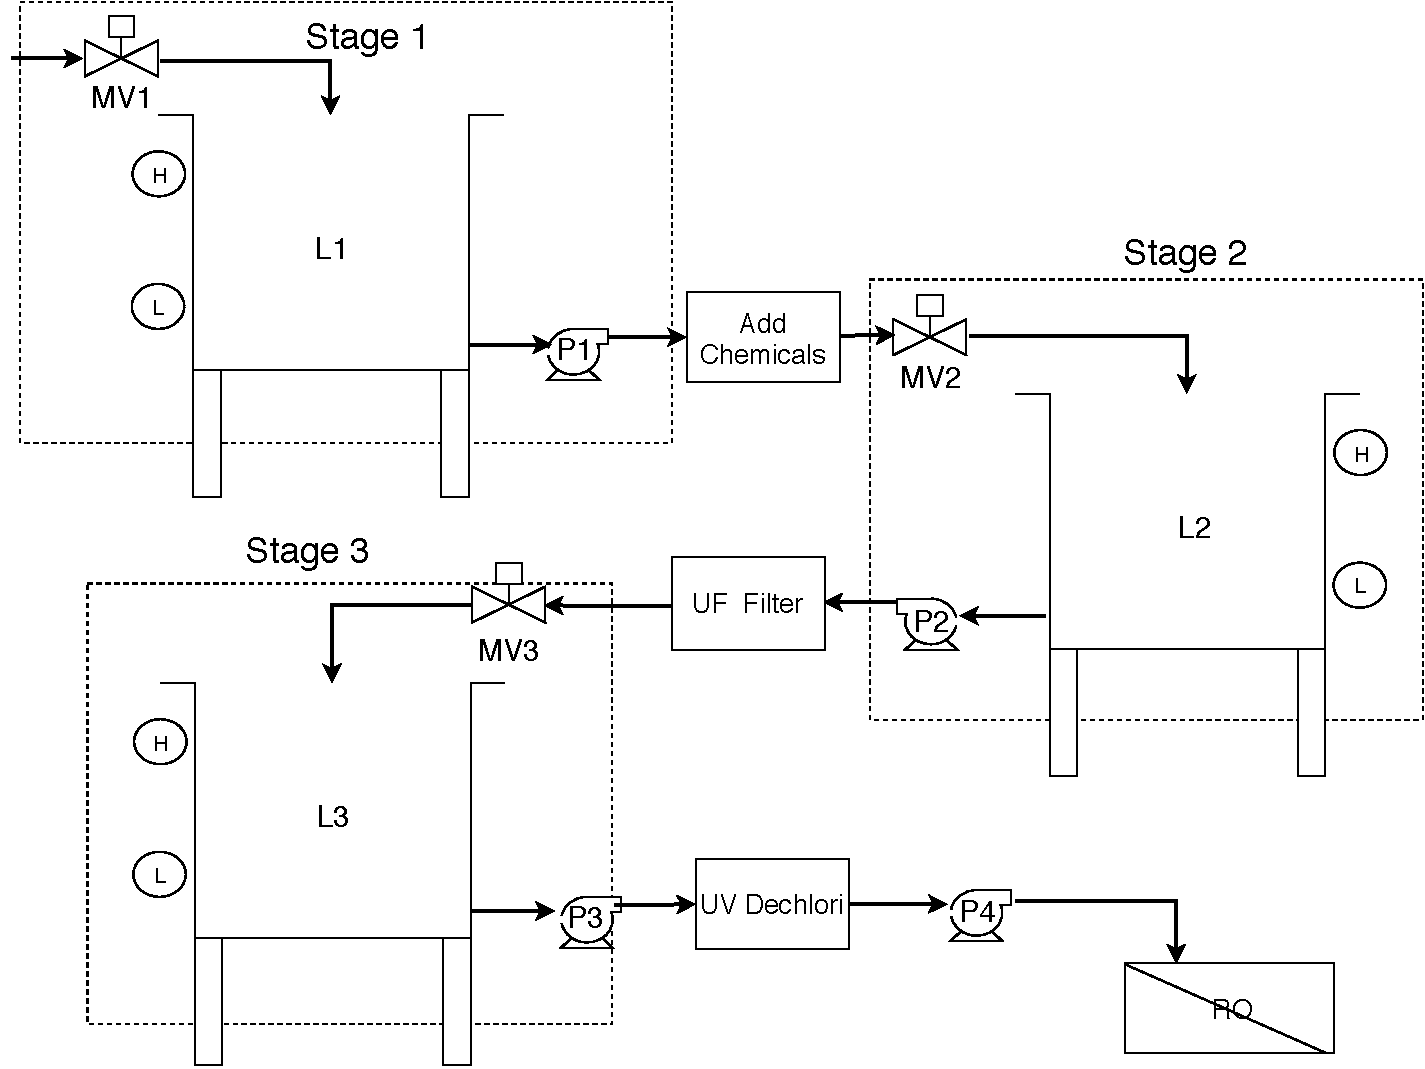
\includegraphics[width=\linewidth]{Figures/SWaT_allTanks-Stages}
  \end{subfigure}
  %
  \begin{subfigure}[b]{.35\linewidth}
  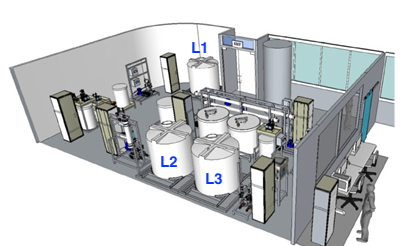
\includegraphics[width=\linewidth]{Figures/testbed.png}
  \end{subfigure}
  %
  \begin{subfigure}[b]{.35\linewidth}
  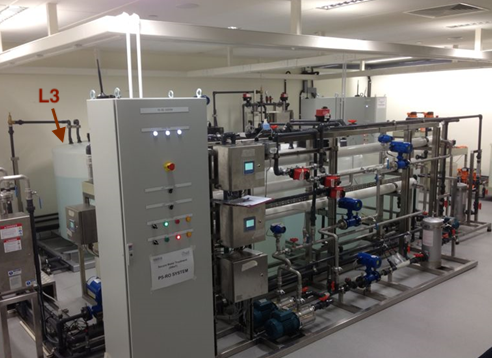
\includegraphics[width=\linewidth]{Figures/testbed2.png}
  \end{subfigure}
  
    \caption{SWaT diagram}
  \label{fig:CPSRobustness:SWaTSchema}
\end{figure}

%==================END JOHN WORKSPACE====================
%==================BEGIN ERIC WORKSPACE====================
\subsection{SWaT Stage 3}
Recall the motivational example presented in Section~\ref{sec:CPSRobustness:example} that models a water tank; such water tank is the Stage 3 submodule of SWaT. We reuse the dynamics presented in Section~\ref{sec:CPSRobustness:example} (which we henceforth refer to as Stage 3), but since there are also pumps and valves in the other process we model, i.e., Stage 2, we rename the components: $MV$, $L$, and $P$ from Section~\ref{sec:CPSRobustness:example} are now respectively $MV3$, $L3$ and $P3$, matching the descriptions in Figure~\ref{fig:CPSRobustness:SWaTSchema}.

Stage 3 receives water from Stage 2, and the controller of Stage 3 reports to the controller of Stage 2 the following information: the level of water in the tank $T3$ and the state of the valve $MV3$. To model the composition of Stage 3 with Stage 2, we define the behaviour of the communication channels $\vec{a}$, and $\vec{w}$ for Stage 2, and $\vec{b}$ and $\vec{v}$ for Stage 3. Let  
\begin{align}
  \vec{b}[L3](k+1)&\triangleq \vec{q}[L3](k)\\
  \vec{b}[MV3](k+1)&\triangleq \vec{q}[MV3](k)\\
  \vec{w}[L2](k)&\triangleq \vec{v}[L2](k),\\
  Inflow(k)&=\begin{cases}
    0 & \quad \text{if $\vec{w}[L2](k)=0$}\\
    0.31,&\quad \text{if $\vec{x}[MV](k)=\texttt{open}$}\\
    0,&\quad \text{if $\vec{x}[MV](k)=\texttt{closed}$}\\
    0.26,&\quad \text{otherwise}\\
  \end{cases}
\end{align}
where $\vec{v}[L2](k)$ is part of the behaviour description of Stage 2. The inflow of water for $T3$ now depends on the physical state of $T2$; if there is no water in $T2$, there is no inflow.

We now formally model Stage 2 and describe its composition with Stage 3. We then characterise an attacker model to measure the robustness of the composition, which we then proceed to redesign and prove that its robustness improves with respect to given the attacker model.

\subsection{A Formal Model of Stage 2}
We provide a model of SWaT Stage 2. This model has three physical components $MV2$, $L2$ and $P2$, and uses the constants $L2min=800$, $L2max=1000$ and $T2=7$.

\paragraph{The Controller $\plc_2$.} 
This controller has eight modes which depend on the state of the pump $P2$ and the valve $MV2$, and a timer, so $\vec{q}$ has three coordinates: $P2$, $MV2$, and $\tau2$. Their respective ranges are 
\begin{align*}
  \vec{q}[P2]&\in\set{\texttt{off},\texttt{on}},\\
  \vec{q}[MV2]&\in\set{\texttt{closed},\texttt{opening},\texttt{open},\texttt{closing}},\\
  \vec{q}[\tau2]&\in\mathbb{N}
\end{align*}

The controller $\plc_2$ receives a network input $\vec{a}$ and a sensor reading $\vec{y}$, and produces a control command $\vec{u}$. Through this section, we assume that every actuator and sensor behaves like a faithful single state transducer, i.e. $\vec{i}(k)=\theta_{\vec{Y}}(\vec{y}(k))=\vec{y}(k)$ and $\vec{u}(k)=\theta_{\vec{O}}(\vec{o}(k))=\vec{o}(k)$. 
The network input $\vec{a}$ has two coordinates $L3$ and $MV3$, whose ranges are 
\begin{align*}
  \vec{a}[L3]&\in[0..1200],\\ 
  \vec{a}[MV]&\in \{\texttt{closed},\texttt{opening},\texttt{open},\texttt{closing}\}.
\end{align*} 
The sensor reading $\vec{y}$ has one coordinate $L2$, where $\vec{y}[L2]\in[0..1200]$. 
The control command $\vec{u}$ has two coordinates, $MV2$ and $L2$, where 
\begin{align*}
  \vec{u}[P2]&\in\set{\const_\texttt{off},\const_\texttt{on},\id},\\
  \vec{u}[MV2]&\in\set{\texttt{closed},\texttt{opening},\const_\texttt{open},\const_\texttt{closing}, \id}.
\end{align*}
%$\vec{u}[MV2]\in\set{\const_\texttt{closed},\const_\texttt{opening},\const_\texttt{open},\const_\texttt{closing}}$.

Let $L3_k=\vec{a}[L3](k)$, $MV3_k=\vec{a}[MV3](k)$, $MV2_k=\vec{q}[MV2](k)$, $P2_k=\vec{q}[P2](k)$, and $L2_k=\vec{y}[L2](k)$; we define the behaviour of the controller PLC2 as follows:
%The controller has the function $\delta_{\vec{Q}}$, defined by
\begin{align}
  % \delta_{\vec{Q}}&((P2,MV2,\tau_2),(L,MV),L2)\triangleq (P2', MV2',\tau_2'),\text{where}\\
\vec{q}[P2](k+1)&\triangleq
    \begin{cases}
      \texttt{off},&\quad \text{if $L3_k\leq L3min$ or $MV3_k\in \set{\texttt{closed},\texttt{closing}}$},\\
      \texttt{on},&\quad \text{if $L3_k \geq L3min$ or $MV3_k\in \set{\texttt{open},\texttt{opening}}$}\\
      P2_k&\quad \text{otherwise;}
    \end{cases}\\
\vec{q}[MV2](k+1)&\triangleq
  \begin{cases}
    \texttt{opening},&\quad \text{if $MV2_k=\texttt{closed}$ and $L2_k\leq L2min$,}\\
    \texttt{open},&\quad \text{if $MV2_k=\texttt{opening}$ and $\tau2_k>T_2$,}\\
    \texttt{closing},&\quad \text{if $MV2_k=\texttt{open}$ and $L2_k\geq L2max$,}\\
    \texttt{closed},&\quad \text{if $MV2_k=\texttt{closing}$ and $\tau2_k>T_2$,}\\
    MV2&\quad \text{otherwise;}    
  \end{cases}\\
\vec{q}[\tau2](k+1)&\triangleq
\begin{cases}
  \tau2_k+1 &\quad \text{if $MV2_k\in \set{\texttt{opening},\texttt{closing}}$}\\
  0&\quad \text{otherwise;}    
\end{cases}\\
\vec{u}[MV2](k+1)=&\const_{MV2_k},\\%\vec{q}[MV2](k)\\%
\vec{u}[P2](k+1)=&\const_{P2_k}.%\vec{q}[P2](k)\\%
\end{align}
% \begin{align*}
%   \theta_{\vec{Q}}(P2,MV2,t)&\triangleq (\vec{o}[MV2],\vec{o}[P2]), \text{where}\\
%   \vec{o}[MV2]&\triangleq MV2
%     % \begin{cases}
%     %   \texttt{open},&\quad  \text{if $MV2=\texttt{opening}$}\\
%     %   \texttt{close},&\quad\text{if $MV2=\texttt{closing}$}\\  
%     %   \perp,&\quad\text{otherwise;}   
%     % \end{cases},
%   ,\quad \text{and }\quad
%   \vec{o}[P2]\triangleq P2
%   % \begin{cases}
%   %   \texttt{on}(),&\quad  \text{if $P2=\texttt{on}$}\\
%   %   \texttt{off}(),&\quad\text{if $P2=\texttt{off}$}\\  
%   %   \perp,&\quad\text{otherwise;}   
%   % \end{cases}
%   \\ 
%   \beta_{\vec{Q}}(P2,MV2,t) &\triangleq \perp.
% \end{align*}
% \paragraph{The Actuators} We have two actuators, the pump $P2$ and the motor valve $MV2$. Their  behaviour is modelled by the function $\theta_{\vec{O}}$, defined for $\vec{o}=(MV2,P2)$ by
% \begin{align}
%   \theta_{\vec{O}}(MV2,P2)&\triangleq (\vec{u}[MV2],\vec{u}[P2]), \text{where}\\
%   \vec{u}[MV2]&\triangleq 
%     \begin{cases}
%       \const_{MV2},&\quad  \text{if $MV2\neq\perp$,}\\
%       \id,&\quad\text{otherwise;}   
%     \end{cases},\\
%   \vec{o}[P2]&\triangleq 
%   \begin{cases}
%     \const_{P2},&\quad  \text{if $P2\neq \perp$,}\\
%     \id,&\quad\text{otherwise;}   
%   \end{cases},
% \end{align}

\paragraph{The Process} 
The state of the process $\vec{x}$ has three coordinates: $L2, MV2$ and $P2$. Their respective ranges are $\vec{x}[L2]\in [0..1200]$, $\vec{x}[MV2]\in \{\texttt{closed},\texttt{opening},\texttt{open},\texttt{closing}\}$ and $\vec{x}[P2]\in \set{\texttt{on},\texttt{off}}$. 
% subcomponents $\vec{x}=(L2,MV2,P2)$, with $\range(\vec{x}[L2])=[0..1200]$, $\range(\vec{x}[MV2])=\set{\texttt{closed},\texttt{opening},\texttt{open},\texttt{closing}}$, and $\range(\vec{x}[P2])=\set{\texttt{on},\texttt{off}}$. 

We leave the initial condition abstract for now. The behaviour of the process is given by
% \todo[inline]{@Eric:The initial state of the process is $\vec{x_0}=(990,\texttt{open},\texttt{on})$.}
%The process reacts to the control input $\vec{u}$,

% The process has the function $\delta_{\vec{X}}$, which computes the of value of $\vec{x}(k+1)$ from $\vec{x}(k)$, $\vec{u}[MV2](k)$ and $\vec{u}[P2](k)$
Let $P2_k=\vec{x}[P2](k)$, $MV2_k=\vec{x}[MV2](k)$, and $L2_k=\vec{x}[L2](k)$, and let $\delta_{P2}=\vec{u}[P2](k)$, and $\delta_{MV2}=\vec{u}[MV2](k)$; we define the behaviour of the process by
\begin{align*}
  %\delta_{\vec{X}}&((L2,MV2,P2),(\vec{u}[MV2],\vec{u}[P2]))\triangleq (L2', MV2',P2'),\text{where}\\
\vec{x}[P2](k+1)&\triangleq \delta_{P2}(P2_k)\\
\vec{x}[MV2](k+1)&\triangleq \delta_{MV2}(MV2_k)\\
\vec{x}[L2](k+1)&\triangleq L2_k+\partial(MV2_k,P2_k),\text{where}\\
\partial(MV2,P2)&\triangleq
\begin{cases}
  0&\quad \text{if $MV2_k=\texttt{closed}$ and $P2_k=\texttt{off}$}\\
  0.46&\quad \text{if $MV2_k=\texttt{open}$ and $P2_k=\texttt{off}$}\\
  0.29&\quad \text{if $MV2_k\in\set{\texttt{opening},\texttt{closing}}$ and $P2_k=\texttt{off}$}\\
  -0.29&\quad \text{if $MV2_k=\texttt{closed}$ and $P2_k=\texttt{on}$}\\
  0.13&\quad \text{if $MV2_k=\texttt{open}$ and $P2_k=\texttt{on}$}\\
  -0.28&\quad \text{if $MV2_k\in\set{\texttt{opening},\texttt{closing}}$ and $P2_k=\texttt{on}$}\\  
\end{cases}
\end{align*}
The values for $\partial(MV2,P2)$ were computed by linear regression to approximate the flow equation $L2_{k+1}=L2_{k}+\texttt{Inflow}_k-\texttt{Outflow}_k$.

The sensor reading $\vec{y}$ has only one coordinate $L2$, whose range is $\vec{y}\in \mathbb{R}^+$; i.e, any positive value. The behaviour of $\vec{y}$ is given by 
\begin{align}
  \vec{y}[L2](k)=\vec{x}[L2]
\end{align}

Finally, the physical state of the process propagates to Stage 3 via the abstract channel $\vec{v}[L3]$
\begin{align}
  \vec{v}[L2](k)&\triangleq \vec{x}[L2](k)
\end{align}
Figure~\ref{fig:CPSRobustness:Stage2Normal} shows the normal steady state behaviour of the water level in tank T2. Due to interdependence, many changes in the behaviour of the tank T2 affect the behaviour of tank T3 and vice versa. 
%\todo[inline]{@John: we are doing testing so it should be fine, but I can imagine a reviewer complaining about the omision of the error parameter. What reasoning can we use to omit explicitly including the error parameter?}

% \todo[inline]{@All. Reviewers might ask why we do not include errors in the models. They can be added, but I wanted to keep the model as simple as possible.}

% The process produces the output $\theta_{\vec{X}}$, defined by
% \begin{align*}
%   \theta_{\vec{X}}(\vec{x})\triangleq \vec{y}[L2], \text{where $\vec{y}[L2]=\vec{x}[L2]$}.
% \end{align*} 
% \paragraph{Sensors} Finally, the behaviour of the water level sensor is given by the function $\theta_{\vec{Y}}$, defined by 
% \begin{align*}
%   \theta_{\vec{Y}}(\vec{y})\triangleq \vec{i}[L2]\text{, where $\vec{i}[L2]=\vec{y}[L2]$.}
% \end{align*}

\begin{figure}[t]
  \centering
  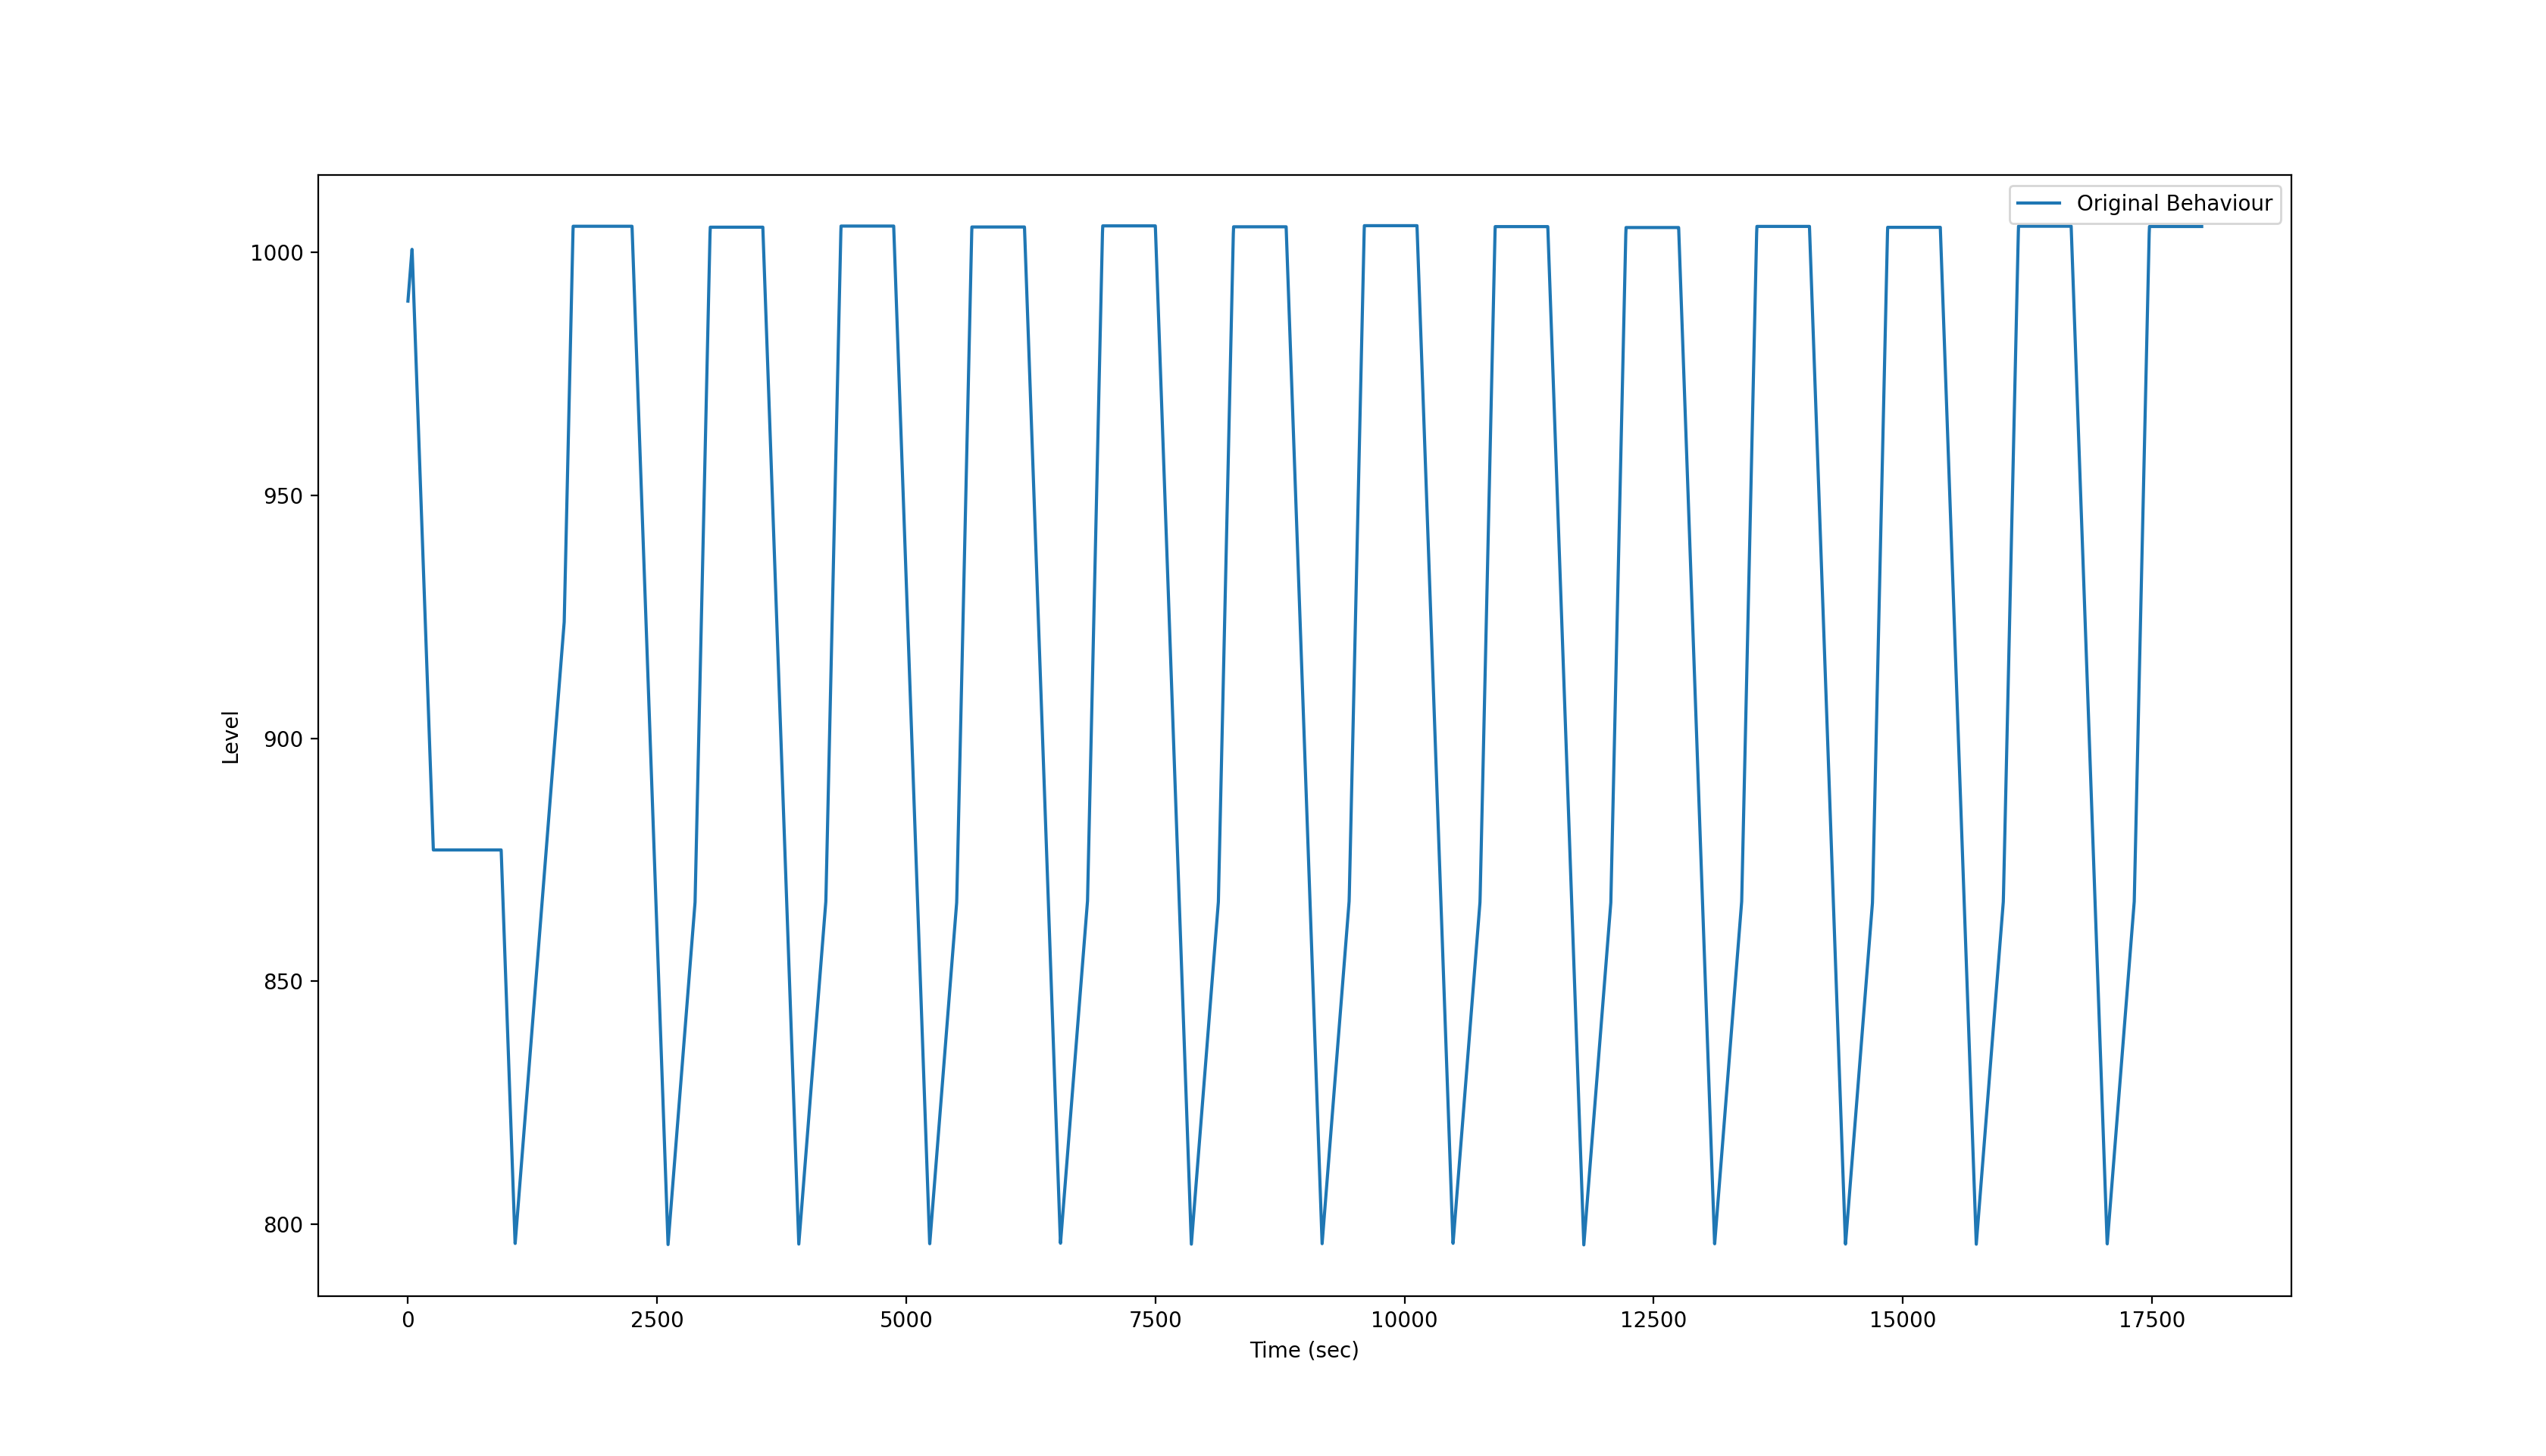
\includegraphics[width=0.75\textwidth]{Figures/Stage2Normal.png}
  \caption{Normal behaviour of the water level of Stage 2 if Stage 3 is also operating normally.}
  \label{fig:CPSRobustness:Stage2Normal}
\end{figure}

% The controller has the output functions $\beta_{\vec{Q}}$ and $\theta_{\vec{Q}}$, defined by
% \begin{align}
%   \theta_{\vec{Q}}(P2,MV2,t)&\triangleq (\vec{o}[MV2],\vec{o}[P2]), \text{where}\\
%   \vec{o}[MV2]&\triangleq 
%     \begin{cases}
%       \texttt{open}(),&\quad  \text{if $MV2=\texttt{opening}$}\\
%       \texttt{close}(),&\quad\text{if $MV2=\texttt{closing}$}\\  
%       \perp,&\quad\text{otherwise;}   
%     \end{cases},\\
%   \vec{o}[P2]&\triangleq P2\\ 
%   \beta_{\vec{Q}}(P2,MV2,t) &\triangleq \perp.
% \end{align}

\subsection{Attacker Model}%{Some Attacker Models of Stage 2 and Stage 3}
% We define an attacker model for the composition of Stage 2 and Stage 3 by combining two attacker models, one for Stage 2 and one for Stage 3.  The following models describe single-point attackers in one of the processes.
We now define an attacker model using Definitions~\ref{def:CPSRobustness:AttackBasis}, \ref{def:CPSRobustness:IdempotentMonoid}, and~\ref{def:CPSRobustness:Attack} for the quantification of robustness. We have four security requirements: $\Always{\vec{x}[L2]>0}$, $\Always{\vec{x}[L2]<1200}$, $\Always{\vec{x}[L3]>0}$ and $\Always{\vec{x}[L3]<1200}$. 
We consider an attacker model that manipulates the control outputs of the controller PLC2 for pump $P2$ and valve $MV2$. We choose this attacker because they can override the commands sent by PLC2, giving them the same level of control than the PLC2. For testing, we allow this attacker to set $\vec{u}[MV2](k)$ and $\vec{u}[P2](k)$ for all $0\leq k\leq t$ given some testing time parameter $t$, which we set to 6 hours to give the effect of actions of the attacker enough time to propagate through the system. To define the attacker model, we reuse the base from Example~\ref{ex:CPSRobustness:AttackBasis}. The base for the attacker model is $[LL, OK, HH]^T$, where ${LL}(\pi)=\pi[\vec{x}[L3]]<L3min$, ${HH}(\pi)=\pi[\vec{x}[L3]]>L3max$ and ${OK}(\pi)=L3min \leq \pi[\vec{x}[L3]]\leq L3max$, for $\pi \in \Pi$. This implies that even though the attacker modifies components in Stage2, they only have visibility of the tank T3 and not of T2. Although this attacker is ``blind" with respect to $T2$, their actions will definitely impact the behaviour of $T2$. The representative values used by the attacker model for $\vec{u}[MV2]$ are $\texttt{open}$ and $\texttt{closed}$; more precisely, we define
\begin{align*}
  \Gamma_{\vec{u}[MV2]}=\set{\const^{\vec{u}[MV2]}_{\texttt{open}}, \const^{\vec{u}[MV2]}_{\texttt{closed}}}.
\end{align*}
The representative values for $\vec{u}[P2]$ are $\texttt{on}$ and $\texttt{off}$, which create the constant functions
\begin{align*}
  \Gamma_{\vec{u}[P2]}=\set{\const^{\vec{u}[P2]}_{\texttt{on}}, \const^{\vec{u}[P2]}_{\texttt{off}}}.
\end{align*}
% The set of coefficients for this attacker model is $\Gamma_{\vec{u}[MV2],\vec{u}[P2]}=\Gamma_{\vec{u}[MV2]}\cup \Gamma_{\vec{u}[P2]}$. 
The attacks of this attacker model $\vec{m}$ are then of the form
\begin{align*}
  \vec{m}(\pi)=
  %[t_1,\ldots,t_n]
  \begin{bmatrix}
    t_{LL}\circ s_{LL} \\
    t_{OK}\circ s_{OK} \\
    t_{HH}\circ s_{HH} \\
  \end{bmatrix}
  \cdot
  \begin{bmatrix}
    LL \\
    OK \\
    HH
  \end{bmatrix},
\end{align*} 
where $t_i\in \set{\id,\const^{\vec{u}[MV2]}_{\texttt{open}}, \const^{\vec{u}[MV2]}_{\texttt{closed}}}$ and  $s_i\in\set{\id,\const^{\vec{u}[P2]}_{\texttt{on}}, \const^{\vec{u}[P2]}_{\texttt{off}}}$, for $i\in \set{LL,OK,HH}$. The resulting attacker model has 729 attacks because
 \begin{align*}
  \left| \IM{\Gamma_{\set{\vec{u}[MV2],\vec{u}[P2]}}}\right|^{\left|\set{{LL},{OK},{HH}}\right|}=9^3=729.
\end{align*}

\subsection{Counterattacker Model}
The corresponding counterattacker model uses the controller PLC3; i.e. the counterattacker can set $\vec{q}[MV3](k)$ and $\vec{q}[P3](k)$ for all $0\leq k\leq t$ , with  $t=6$ hours to let the actions of the attacker and counterattacker enough time to stabilise. Since the counterattacker is in the controller of Stage 3, we define the base for the counterattacker model to be $[LL', OK', HH']^T$, where ${LL'}(\pi)=\pi[\vec{y}[L3]]<L3min$, ${HH'}(\pi)=\pi[\vec{y}[L3]]>L3max$ and ${OK'}(\pi)=L3min \leq \pi[\vec{y}[L3]]\leq L3max$, for $\pi \in \Pi$ (unlike the base of the attacker, which uses $\vec{x}[L3]$ instead of $\vec{y}[L3]$). The counterattacker is also ``blind" with respect to $T2$, but their actions also impact the behaviour of $T2$. 

We set the representative values of $\vec{q}[MV3]$ to be $\texttt{open}$, and $\texttt{closed}$ and the representative values of $\vec{q}[P3]$ to be $\texttt{on}$, and $\texttt{off}$; more precisely, 
\begin{align*}
  \Gamma_{\vec{q}[MV3]}&=\set{\const^{\vec{q}[MV3]}_{\texttt{open}}, \const^{\vec{q}[MV3]}_{\texttt{closed}}}.\\
  \Gamma_{\vec{q}[P3]}&=\set{\const^{\vec{q}[P3]}_{\texttt{on}}, \const^{\vec{q}[P3]}_{\texttt{off}}}.
\end{align*}
% The set of coefficients for this attacker model is $\Gamma_{\vec{u}[MV2],\vec{u}[P2]}=\Gamma_{\vec{u}[MV2]}\cup \Gamma_{\vec{u}[P2]}$. 
The counterattacks of this model $\vec{w}$ are then of the form
\begin{align*}
  \vec{w}(\pi)=
  %[t_1,\ldots,t_n]
  \begin{bmatrix}
    t_{LL'}\circ s_{LL'} \\
    t_{OK'}\circ s_{OK'} \\
    t_{HH'}\circ s_{HH'} \\
  \end{bmatrix}
  \cdot
  \begin{bmatrix}
    LL' \\
    OK' \\
    HH'
  \end{bmatrix},
\end{align*} 
where $t_i\in \set{\id,\const^{\vec{q}[MV3]}_{\texttt{open}}, \const^{\vec{q}[MV3]}_{\texttt{closed}}}$ and  $s_i\in\set{\id,\const^{\vec{u}[P3]}_{\texttt{on}}, \const^{\vec{u}[P3]}_{\texttt{off}}}$, for $i\in \set{LL',OK',LL'}$. This counterattacker model has 729 counterattacks.

% \begin{figure}[t]
%   \includegraphics[width=0.75\textwidth]{Figures/CounterAtkRank.pdf} 
%   \caption{Counterattack ranking}
%   \label{fig:CPSRobustness:CounterAtkRanking}
% \end{figure}


\subsection{Quantification of Robustness: Analysis of Results}
Using LBA, we quantify the robustness of the system given the initial conditions $\vec{x}[L2]=990$, $\vec{x}[MV2]=open$, $\vec{x}[P2]=on$, $\vec{x}[L3]=920$, $\vec{x}[MV3]=open$, $\vec{x}[P3]=on$. The robustness factor of 162/729, meaning that are successful 567 attacks for the given attacker model. All attacks that break $\Always{\vec{x}[L3]>0}$ or $\Always{\vec{x}[L3]<1200}$ can always be countered. However, 136 attacks cannot be countered by the proposed counterattacker model, meaning that the latent robustness of the system is only $593/729$. Non countered attacks always break either $\Always{\vec{x}[L2]>0}$ or $\Always{\vec{x}[L2]<1200}$. Nevertheless, some attacks which break $\Always{\vec{x}[L2]>0}$ or $\Always{\vec{x}[L2]<1200}$ can be countered. For example, the attack
\begin{align*}
%   Requirement "Tank T2 Never Overflows" broken at time 644 by attack (x[L3]<L3min)=>[(O[P2]->off), (O[MV2]->open)] + (L3min<=x[L3]<=L3max)=>[id(O[P2]), id(O[MV2])] + (x[L3]>L3max)=>[id(O[P2]), id(O[MV2])]
% Found counterattack(Y[L3]>L3max)=>[id(Q[MV3]), (Q[P3]->off)] + (L3min<=Y[L3]<=L3max)=>[id(Q[MV3]), id(Q[P3])] + (Y[L3]<L3min)=>[id(Q[MV3]), id(Q[P3])]
  \vec{m}(\pi)&=
  %[t_1,\ldots,t_n]
  \begin{bmatrix}
   \const^{\vec{u}[MV2]}_{\texttt{open}}\circ \const^{\vec{u}[P2]}_{\texttt{off}} \\
   \id\circ \id \\
   \id\circ \id \\
  \end{bmatrix}
  \cdot
  \begin{bmatrix}
    \pi[\vec{x}[L3]]<L3min \\
    L3min \leq \pi[\vec{x}[L3]]\leq L3max \\
    \pi[\vec{x}[L3]]>L3max
  \end{bmatrix},
\end{align*} 
breaks the requirement $\Always{\vec{x}[L2]<1200}$, but it is countered by the counterattack 
\begin{align*}
  \vec{w}(\pi)&=
  %[t_1,\ldots,t_n]
  \begin{bmatrix}
    \id\circ \id \\
    \id\circ \id \\
    \id\circ \const^{\vec{q}[P3]}_{\texttt{off}} \\
  \end{bmatrix}
  \cdot
  \begin{bmatrix}
    \pi[\vec{y}[L3]]<L3min \\
    L3min \leq \pi[\vec{y}[L3]]\leq L3max \\
    \pi[\vec{y}[L3]]>L3max
  \end{bmatrix}.
\end{align*} 
The counterattack works by preventing the conditions that trigger the attack; more precisely, the attack activates when $\pi[\vec{x}[L3]]<L3min$, and the counterattack $\vec{w}$ prevents such condition from happening (although the behaviour eventually causes the system to reach a state where water does not flow in or out of the tanks). 

The following attack
\begin{align*}
  %(x[L3]<L3min)=>[id(O[P2]), id(O[MV2])] + (L3min<=x[L3]<=L3max)=>[(O[P2]->off), (O[MV2]->open)] + (x[L3]>L3max)=>[(O[P2]->off), id(O[MV2])]
    \vec{m}'(\pi)&=
    %[t_1,\ldots,t_n]
    \begin{bmatrix}
     \id\circ \id \\
     \const^{\vec{u}[MV2]}_{\texttt{open}}\circ \const^{\vec{u}[P2]}_{\texttt{off}} \\
     \id\circ \const^{\vec{u}[P2]}_{\texttt{off}} \\
    \end{bmatrix}
    \cdot
    \begin{bmatrix}
      \pi[\vec{x}[L3]]<L3min \\
      L3min \leq \pi[\vec{x}[L3]]\leq L3max \\
      \pi[\vec{x}[L3]]>L3max
    \end{bmatrix}
  \end{align*} 
causes tank T2 to overflow, and it cannot be countered using the current counterattacker model. This and similar attacks cannot be countered because the controller of Stage 3 cannot compensate the effects of an attacker controlling $\vec{u}[MV2]$ by influencing other components. 

\subsection{Increasing Robustness}
%\todo[inline]{Discuss a couple of attack and counterattack dynamics, several counterattacks vs several attacks with some things in common.}
Using LBA, we can group attacks that are countered by the same counterattack. After evaluating the composition of Stage 2 and Stage 3 under the given attacker and counterattacker models, we observe 12 counterattacks to address 431 successful attacks. The number of attacks countered by each counterattack does not follow a uniform distribution; some counterattacks counter only a couple of attacks, while others counter hundreds. 

For a given counterattack $\vec{w}$ which counters $n$ attacks $\vec{m}_1, \ldots, \vec{m}_n$, understanding the similarities among the $n$ attacks gives us a good indication of the reason why the counterattack is effective. For this evaluation, we manually analysed possible common causes, but a more systematic and efficient methodology is encouraged for future work. In summary, we identified 333 attacks that cause T2 to overflow, 126 that cause T2 to empty and 108 that cause T3 to empty; no attack caused T3 to overflow because we stop analysis at the first cause of problem, and attacks that can overflow T3 can also overflow T2, empty T2 or empty T3 faster than they can overflow T3.


\subsubsection{A Correct Repair}
\label{sec:CPSRobustness:CorrectRepair}
For an attack $\vec{m}$ and a counterattack $\vec{w}$ which counters it, if we implement the composition $\vec{w}\circ \vec{m}$, this transformation does not break the requirements of the system, although it may take the system to exceptional states. In general, implementing the application of a counterattack is far from trivial: the counterattack must only be applied when an attack it counters is detected; otherwise, the counterattack itself may become an attack! 

In Section~\ref{sec:CPSRobustness:UrgentAttacker}, we mentioned that to implement a counterattack, we must ensure that it is only applied when the attack it counters exists in the system. This implicitly assumes the existence of a system monitor that can correctly identify which attack is being applied to the system; i.e., it properly identifies $\vec{m}$. Once $\vec{m}$ is identified, the monitor applies the appropriate counterattack for $\vec{m}$. Given that this requitements over the monitor are quite restrictive, we explore in the following a different approach: we directly modify the program of a controller PLC, and we run LBA to measure the robustness of the new system to check if it improved. 

We used a counterattacker model which acts on the coordinates $\vec{q}[MV3]$ and $\vec{q}[P3]$ which are normally controlled by controller PLC3. Our plan then is to incorporate a counterattack $\vec{w}$ as part of the program of PLC3. Two parts are necessary: the conditions that would trigger the application of the counterattack, and the right effects over $\vec{q}[MV3]$ and $\vec{q}[P3]$. We observe that several attacks that empty tank T3 can be countered by means of the counterattack 
\begin{align*}
  %(Y[L3]>L3max)=>[id(Q[MV3]), (Q[P3]->off)] + (L3min<=Y[L3]<=L3max)=>[id(Q[MV3]), id(Q[P3])] + (Y[L3]<L3min)=>[id(Q[MV3]), id(Q[P3])]
    \vec{w}(\pi)&=
    %[t_1,\ldots,t_n]
    \begin{bmatrix}
    \id\circ \const^{\vec{q}[P3]}_{\texttt{off}} \\
     \id\circ \id \\
     \id\circ \id \\
    \end{bmatrix}
    \cdot
    \begin{bmatrix}
      \pi[\vec{y}[L3]]<L3min \\
      L3min \leq \pi[\vec{y}[L3]]\leq L3max \\
      \pi[\vec{y}[L3]]>L3max
    \end{bmatrix},
  \end{align*} 
which is sensible: if the tank $T3$ is losing water, by shutting off the pump $P3$ when the level is low, we prevent water from leaving the tank. The counterattack $\vec{w}$ counters 122 attacks in total.

The counterattack $\vec{w}$ defines the effects over $\vec{q}[MV3]$ and $\vec{q}[P3]$ to be triggered by the controller PLC3: do nothing with respect to $\vec{q}[MV3]$ and set $\vec{q}[P3]$ to $\texttt{off}$ only if $\pi[\vec{y}[L3]]<L3min$. We now need to establish the conditions that would trigger these effects, and for that we look at common elements among the attacks countered by $\vec{w}$. We observe among several of those attacks that they share the factor $(\const^{\vec{u}[P2]}_{\texttt{off}})(\vec{x}[L3]]<L3min)$; this provides the trigger condition for the application of the effects given by $\vec{w}$.More precisely, to implement the counterattack $\vec{w}$ as part of the controller PLC3, we change its program to set $\vec{q}[P3]$ to \texttt{off} if $\vec{u}[P2]$ is \texttt{off} and $\vec{y}[L3]]<L3min$; we use $\vec{y}[L3]]<L3min$ instead of $\vec{x}[L3]]<L3min$ because $\vec{y}[L3]=\vec{x}[L3]$, because PLC3 has access to $\vec{y}[L3]$, and because the attacker model does not include the coordinate $\vec{y}[L3]$. 

After implementing these changes, we run LBA again. We see that the changes to PLC3 increase the robustness of the system from $162/729$ to $333/729$, since the controller PLC3 now prevents the tank T3 from running out of water due to the effect of 171 previously successful attacks. We recall that $\vec{w}$ countered 122 attacks according to the original LBA, so the change to the program of PLC3 is more profound than anticipated. Nevertheless, the increase in robustness indicates that the system is now more robust after the change, even if the latent robustness remains the same, $593/729$. 

%  that broke this requirement in the original system. The latent robustness remains at 581/729, which means that implementing this counterattack did not add additional vulnerabilities.
 
\subsubsection{A Non-Repair} 
\label{sec:CPSRobustness:NonRepair} We now explore the effects of a modification to the program of PLC3 that does not improve the overall robustness of the system; i.e. a non-repair. The counterattack 
\begin{align*}
%(Y[L3]>L3max)=>[(Q[MV3]->open), id(Q[P3])] + (Y[L3]<L3min)=>[id(Q[MV3]), id(Q[P3])] + (L3min<=Y[L3]<=L3max)=>[id(Q[MV3]), id(Q[P3])] counters the following 42 attacks:
    \vec{w'}(\pi)&=
    %[t_1,\ldots,t_n]
    \begin{bmatrix}
     \id\circ \id \\
     \const^{\vec{q}[MV3]}_{\texttt{open}}\circ \id \\
     \id\circ \id \\
     %\const^{\vec{q}[MV3]}_{\texttt{open}}\circ \id
    \end{bmatrix}
    \cdot
    \begin{bmatrix}
      \pi[\vec{y}[L3]]<L3min \\
      L3min \leq \pi[\vec{y}[L3]]\leq L3max \\
      \pi[\vec{y}[L3]]>L3max
    \end{bmatrix},
  \end{align*} 
%\todo[inline]{Python keeps playing tricks: sometimes it uses this as a counterattack, sometimes it finds another. it's driving me mad.}
counters 58 attacks, many of which overflow T2 and have a common factor of $(\vec{x}[L3]>L3max)\const^{\vec{u}[P2]}_{\texttt{on}}$, i.e., many attacks turn on the pump $P2$ then the level of tank $L3$ is beyond the safety limit $L3max$. 
%\todo[inline]{@John: What happens when the pump is on and the valve is closed? Where does the water go? Reviewers might ask.}
\begin{figure}[t]
  \centering
  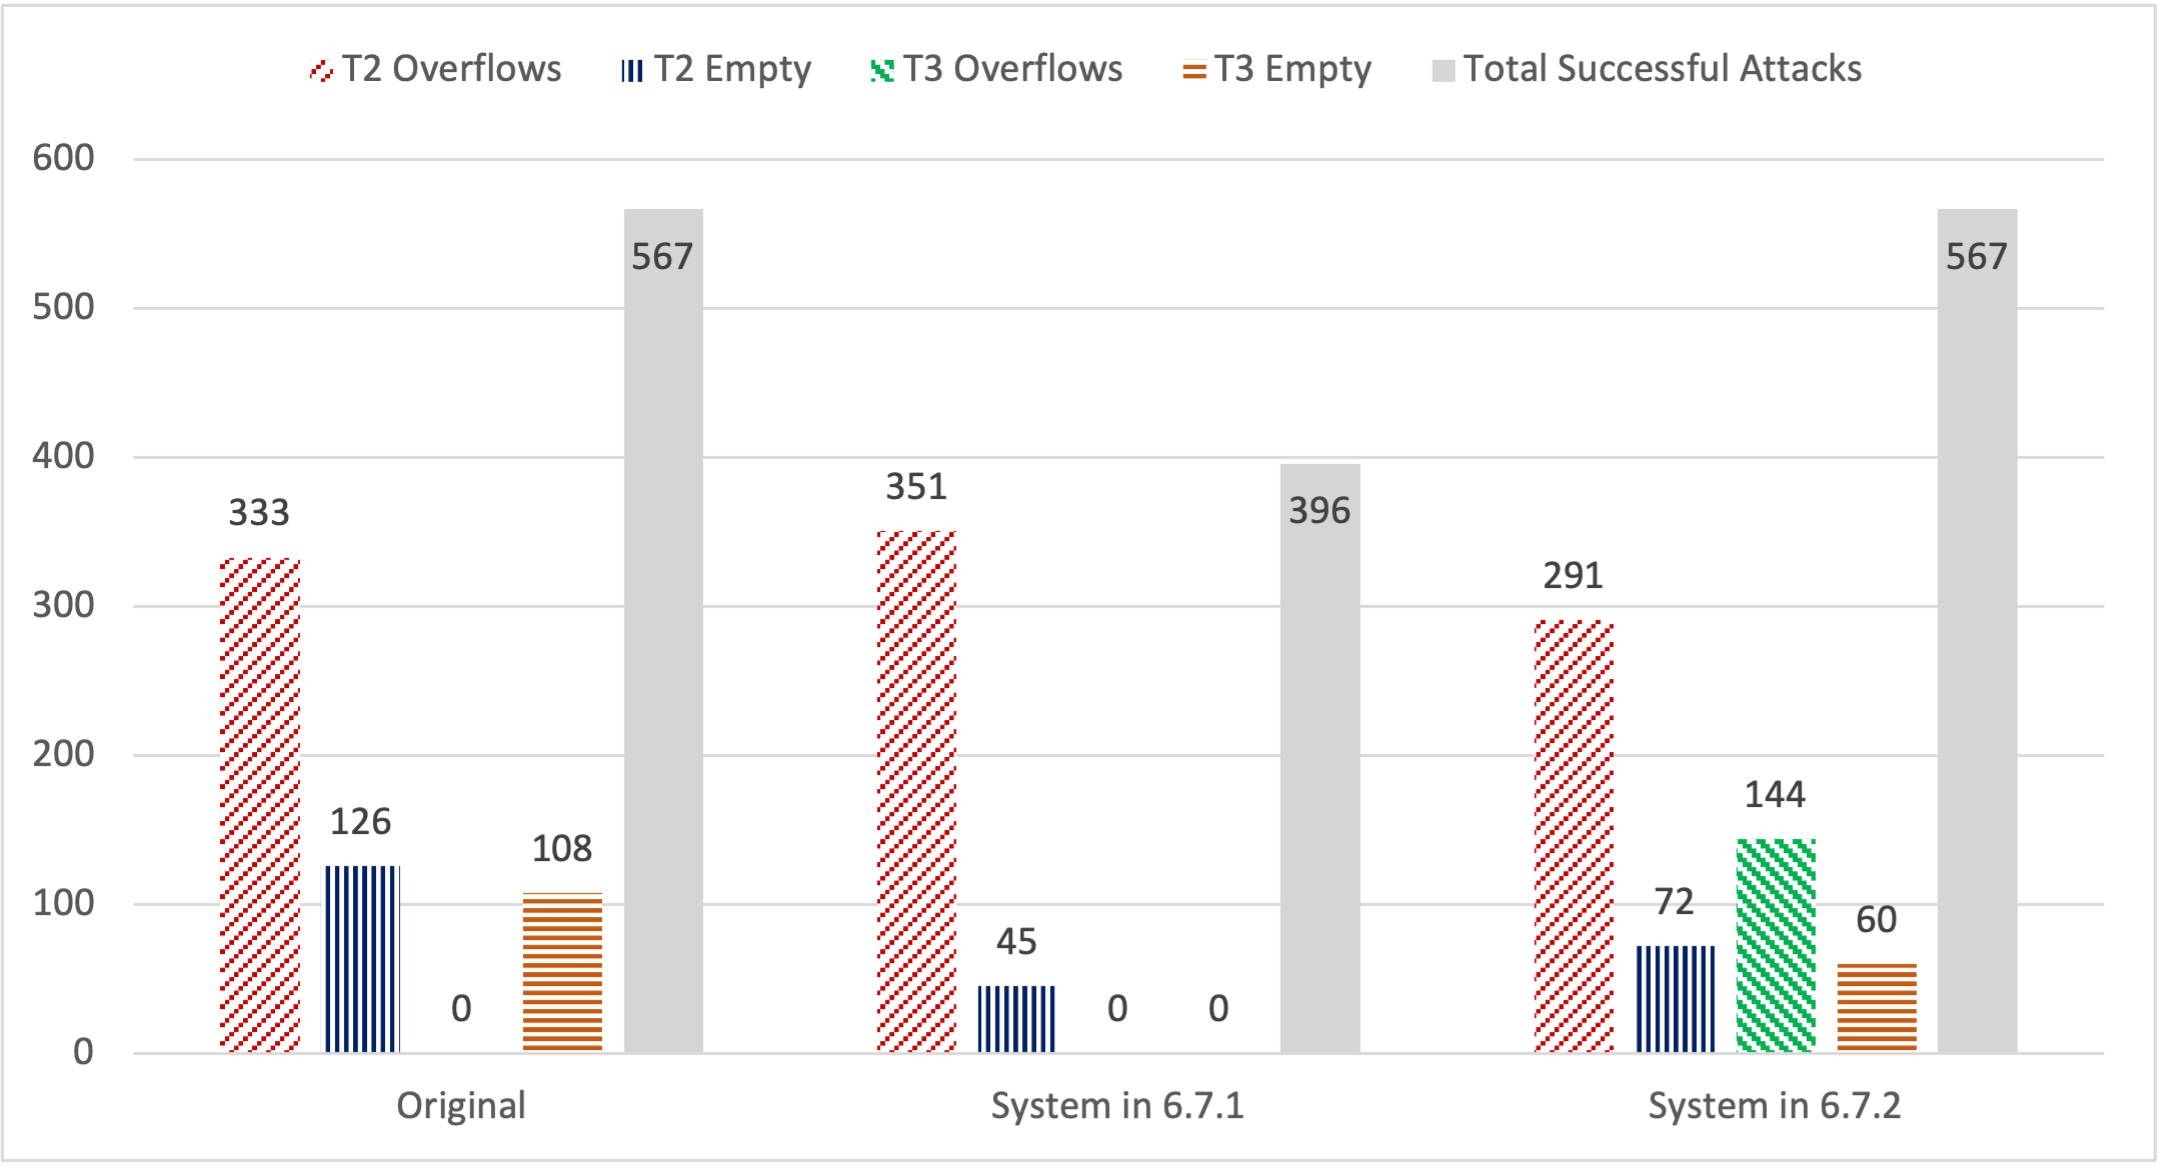
\includegraphics[width=0.75\textwidth]{Figures/AttackDistribution.png} 
  \caption{Attack distribution with respect to the first broken requirement for the original system, the repaired system from Section~\ref{sec:CPSRobustness:CorrectRepair} and the non-repaired system from Section~\ref{sec:CPSRobustness:NonRepair}}
  \label{fig:CPSRobustness:AttackDistribution}
\end{figure} 
Since the condition of the attacks $(\vec{x}[L3]>L3max)$ does not match the condition of the counterattack $L3min \leq \pi[\vec{y}[L3]]\leq L3max$, we just create a rule in the controller that implements the counterattack $\vec{w'}$. To check if such modification improved robustness, we perform LBA, and we observe that the robustness factor remains the same at 162/729; i.e., this new system can also withstand the effect of 162 attacks.  We observe two major differences: the latent robustness of the system changed from 593/729 to 606/729, and the distribution of attacks with respect to the first requirement they break also changes, as shown in Figure~\ref{fig:CPSRobustness:AttackDistribution}. The robustness of the new system is equal to the original robustness, so we cannot consider this to be an improvement over the previous version of the system, which is why we affirm this modification is an example of a non-repair. While this modification reduced the number of attacks that overflow tank T2, it now enables attacks that overflow tank T3, which were previously inexistent. More precisely, in the original system, no attack caused T3 to overflow, but now there are 144 attacks whose first broken requirement is to overflow tank T3. An increase in latent robustness indicates that more attacks in this new system can be countered. This vaguely indicates that the \emph{security potential} increased with respect to the given attacker and counterattacker model.

% Figure \ref{fig:CPSRobustness:AttackDistribution} shows the distribution of attacks for all three systems. Both the original and the non-repaired system have the same number of successful attacks, although their distribution changes.


\subsection{Discussion of Results}
We can use LBA and a testing methodology (e.g., simulation) to check if an arbitrary modification enhances the robustness of the system by comparing the resulting robustness factor. 
We propose two changes to the original Stage 2 and Stage 3 system; one is a repair since it strictly improves the robustness of the system, while the other is not since it only changes the distribution of successful attacks. We believe that a more systematic analysis of the large amounts of data obtained via LBA can produce meaningful suggestions for correct model repairs, e.g., we believe that using machine learning or clustering techniques to find common causes of attacks that are countered by the same counterattack, or finding similarities among counterattacks for the same types of requirements might help the implementation of both system monitors and repairs. 

\begin{figure}[t]
  \centering
  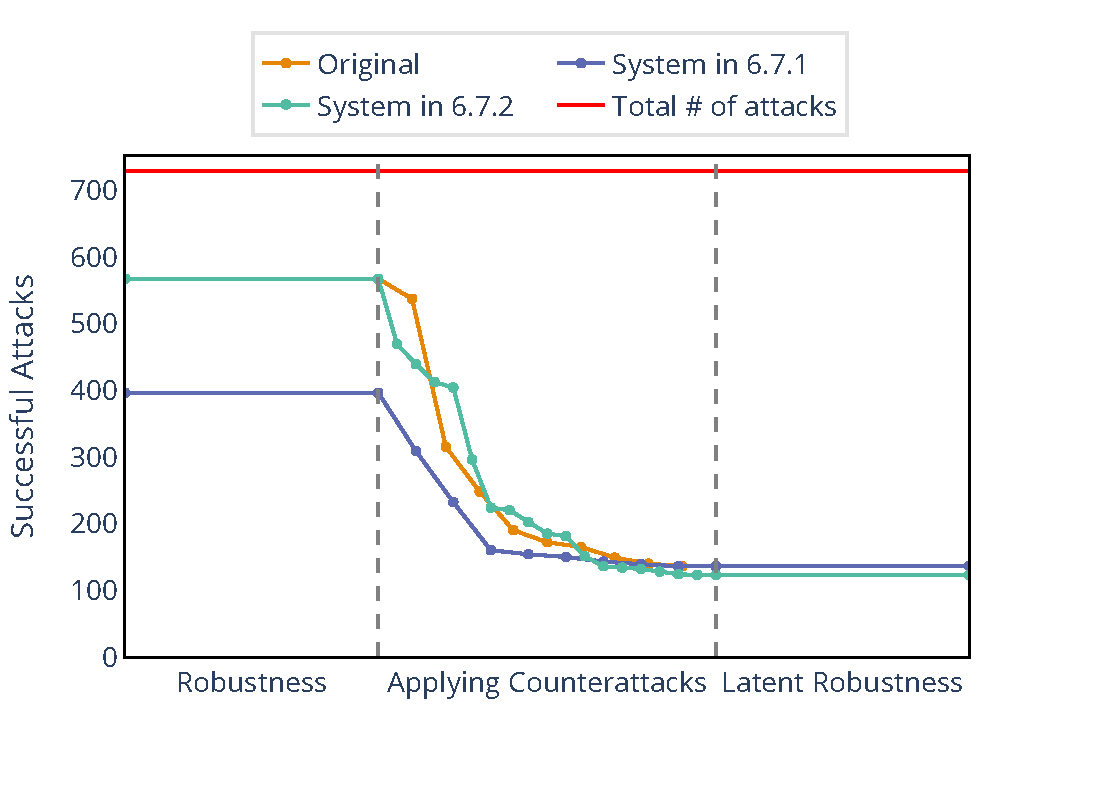
\includegraphics[width=0.75\textwidth]{Figures/Robustness.pdf} 
  \caption{Robustness improvement. The implementation of counterattacks improves the robustness of the system, making it susceptible to fewer attacks.}
  \label{fig:CPSRobustness:Robustness}
\end{figure}
Figure ~\ref{fig:CPSRobustness:Robustness} shows a transition from the robustness innate to the systems presented in this section and their latent robustness. This transition assumes that counterattacks are properly implemented, and that an adequate attack identification monitor exists. A properly implemented counterattack reduces the number of successful attacks, which in turn increases the robustness of the system. Each dot in the ``applying counterattacks'' section corresponds to the cumulative reduction of successful attacks by the proper implementation of a counterattacks that we identified using LBA. By proper implementation of counterattacks, we do not imply that we incorporate them all as part of the normal functionality of the system; instead, that they only activate when it is adequate in an exceptional reactive mode of the system. The slight difference in latent robustness is due to the fact that the original system and the system in Section~\ref{sec:CPSRobustness:NonRepair} are different, and the latter has more attacks that can be countered under the current attacker/counterattacker models. 

For this experiment, we used a very basic counting unweighted metric for robustness that assumes all requirements are equally important. We can refine the definitions of robustness and latent robustness from Definitions~\ref{def:CPSRobustness:Robustness} and \ref{def:CPSRobustness:LatentRobustness} metrics to represent a larger lack of robustness if a particular security requirement is broken by many attacks. 

%, similar to the repair presented in Section ~\ref{sec:CPSRobustness:CorrectRepair}.

% We implement the counterattack $\vec{w'}$ similarly to how we implemented $\vec{w}$: we change the program of PLC3 such that so that, under common conditions given by the countered attacks, we apply the changes indicated by the counterattack $\vec{w'}$. More precisely, PLC3 now sets $\vec{q}[MV3]$ to \texttt{open} if $\pi[\vec{y}[L3]]>L3max$, but it only responding to the factor $(\const^{\vec{u}[P2]}_{\texttt{on}})(\vec{x}[L3]]<L3min)$. Clearly, both $\vec{x}[L3]]<L3min$ and $\pi[\vec{y}[L3]]>L3max$ are mutually exclusive, so this repair does nothing. 

% (Y[L3]>L3max)=>[id(Q[MV3]), (Q[P3]->off)] + (L3min<=Y[L3]<=L3max)=>[id(Q[MV3]), id(Q[P3])] + (Y[L3]<L3min)=>[id(Q[MV3]), id(Q[P3])]
% because
%  \begin{align*}
%   \left| \IM{\Gamma_{\set{\vec{u}[MV2],\vec{u}[P2]}}}\right|^{\left|\set{{LL},{OK},{HH}}\right|}=9^3=729.
% \end{align*}

% \begin{align*}
%   \vec{m}=&(x[L3]<L3min)(\gamma_1(\vec{u}[P2]), \gamma_1(\vec{u}[P2]) + \\
%   &(L3min\leq x[L3]leq L3max)(\gamma_2(\vec{u}[P2]), \gamma_2(\vec{u}[P2]) + \\
%   &(x[L3]>L3max)(\gamma_3(\vec{u}[P2]), \gamma_3(\vec{u}[P2])
% \end{align*}
% % We are mostly interested in discovering attackers that can affect the physical state $\vec{x}$ without physical interaction. We cannot effectively defend from the cyber part of the CPS (e.g. by redesigning the controller, or by adding more sensors) against attackers that can directly manipulate the physical state, because their attackers can bypass the controller. Therefore, we assume that we can protect the physical components of a CPS though physical security, and we assume that attackers are not able to directly corrupt physical component%(i.e. $\vec{u}, \vec{x}, \vec{y}, \vec{v}$ and $\vec{w}$)
% % , so their attacks must be carried out by corrupting non-physical components.% (i.e. $\vec{a}, \vec{b},\vec{i}, \vec{q}$ and $\vec{o}$).

% More precisely,  
% %if the state of a CPS has vectors $\vec{a},\vec{b},\vec{i},\vec{o}, \vec{u}, \vec{y}, \vec{v},\vec{w},\vec{q}$, and $\vec{x}$,
% we define attackers for this CPS over the following set of components 
% \begin{align}
%   \Sigma_{0}=\set{\vec{i}[L2], \vec{a}[L], \vec{a}[MV], \vec{q}[P2], \vec{q}[MV2], \vec{q}[\tau_2], \vec{o}[MV2], \vec{o}[P2]}.
% \end{align}
% We define the partition of states $\set{(L2< L2min),(L2min\leq L2\leq L2max),(L2>L2max)}$ to allow the definition of attacks based on these three predicates over states as explained in Definition~\ref{def:CPSRobustness:Attack}. 

% We chose arbitrary ranges for the vulnerable components in $\Sigma_0$ so that they can have different effects on the controller. For example, $\widehat{\vec{i}[L2]}\triangleq\set{700,900,1100}$, since we evaluate whether $L2 \leq L2min$ and $L2 \geq L2max$, and $L2min=800$ and $L2max=1000$. The ranges for all the vulnerable components are the following:
% \begin{align*}
%   \widehat{\vec{i}[L2]}&\triangleq\set{700,900,1100}\\
%   \widehat{\vec{a}[L]}&\triangleq\set{700,900,1100}\\
%   \widehat{\vec{a}[MV]}&\triangleq\range(\vec{a}[MV])\\ 
%   \widehat{\vec{q}[P2]}&\triangleq\range(\vec{q}[P2])\\
%   \widehat{\vec{q}[MV2]}&\triangleq\range(\vec{q}[MV2])\\
%   \widehat{\vec{q}[\tau_2]}&\triangleq\set{0,7}\\
%   \widehat{\vec{o}[MV2]}&\triangleq\range(\vec{o}[MV2])\\
%   \widehat{\vec{o}[P2]}&\triangleq\range(\vec{o}[P2]).
%   %\set{ \vec{a}[L], \vec{a}[MV], \vec{q}[P2], \vec{q}[MV2], \vec{q}[\tau_2], \vec{o}[MV2], \vec{o}[P2]}.
% \end{align*} 
% Let us first consider attacks that affect only one component. 
% Under this configuration, we generate 1161 attacks on individual components. We present the manifested latent behaviours of these attacks that can break either of the requirements $\Always{\vec{x}[L2]>0}$ or $\Always{\vec{x}[L2]<1200}$ in Figure~\ref{fig:CPSRobustness:DangerousLatentBehavioursStage2}. 
% \begin{figure}[t]
%   \includegraphics[width=\textwidth]{Figures/LevelT2-Stage2Attackers-OnlySuccessfulAttacks-OverUnderflowL2-3Partition.png}
%   \caption{Latent behaviours manifested by attacks on the components of Stage 2. All these latent behaviours break either the overflow or the empty tank requirement.}
%   \label{fig:CPSRobustness:DangerousLatentBehavioursStage2}
%   \end{figure}

% \todo[inline]{
%   Successful attackers with only one component= ${'PLC2[timer]', 'PLC2[mode]', 'O[MV2]', 'L2[level]'}$Analysis finished in 399.3336 seconds.
%   There are 393 successful attacks under state partition ${'L2>L2max', 'L2<L2min', 'L2min<=L2<=L2max'}$
% Tested 1161 attacks in total
% }

% Both Stage 2 and Stage 3 have invariant security requirements: their respective tanks must never be empty and the tanks must never overflow. 

% \subsubsection{Attacking Stage 2}.

% \subsubsection{Attacking Stage 2 from Stage 3}. The results are interesting. There are NO invariant attacks from stage 3 to stage 2, but there are a couple of conditional attacks! The following attacks work because the state of MV sent to Stage 2 depends on the mode of PLC3, and that is what the attacker changes. 
% \begin{itemize}
%   \item stop condition T2\_overflow triggered at time 20658 for attack P.Q[mode]=(L2<L2min)=>id, (L2>L2max)=>(=open), (L2min<=L2<=L2max)=>(=open), 
%   \item stop condition T2\_overflow triggered at time 20657 for attack P.Q[mode]=(L2<L2min)=>id, (L2>L2max)=>(=opening), (L2min<=L2<=L2max)=>(=open), 
%   \item stop condition T2\_overflow triggered at time 20658 for attack P.Q[mode]=(L2<L2min)=>(=closing), (L2>L2max)=>(=open), (L2min<=L2<=L2max)=>(=open), 
%   \item stop condition T2\_overflow triggered at time 20657 for attack P.Q[mode]=(L2<L2min)=>(=closing), (L2>L2max)=>(=opening), (L2min<=L2<=L2max)=>(=open), 
%   \item stop condition T2\_overflow triggered at time 20658 for attack P.Q[mode]=(L2<L2min)=>(=closed), (L2>L2max)=>(=open), (L2min<=L2<=L2max)=>(=open), 
%   \item stop condition T2\_overflow triggered at time 20657 for attack P.Q[mode]=(L2<L2min)=>(=closed), (L2>L2max)=>(=opening), (L2min<=L2<=L2max)=>(=open), 
% \end{itemize}

% \todo[inline]{
%   There are 6 successful attacks under state partition {'L2<L2min', 'L2>L2max', 'L2min<=L2<=L2max'}
% Tested 341 attacks in total
% We tested these attackers= {'PLC3[mode]', 'PLC3[timer]', 'O[MV]', 'L[level]'}
% Successful attackers with only one component= {'PLC3[mode]'}
% Analysis finished in 189.1896 seconds
% }

%==================END ERIC WORKSPACE====================

\section{Discussion and Future Work}
\label{sec:CPSRobustness:Discussion}
In this section, we list and discuss some fundamental discussion points, some of which represent the basis for interesting future work. 
%LBA is a systematic way to test transition systems with respect to a set of properties
%\todo[inline]{We do not work with attackers that act on physical components.}
%\todo[inline]{We do not provide heuristics to choose the most pressing attacker to be addressed.}
\subsection{Modelling and Abstraction level}
Although we provide a formal framework for the modelling of CPSs, their states, and their execution semantics, and showed evidence that it can be used to derive useful analysis, it will be a subject of future work to assess how appropriate our modelling is when applied to other, perhaps more complex, scenarios. In essence, our formalism defines a deterministic transition system whose transition function is given by the one-step cycle semantics function $\TheSystem$ (see Definition \ref{def:CPSRobustness:SingleCycleSemantics}). Consequently, the notion of robustness and latent robustness that we give in Definitions \ref{def:CPSRobustness:Robustness} and \ref{def:CPSRobustness:LatentRobustness} are not probabilistic. However, we believe that this approach is good enough to carry out an approximate analysis if the probabilistic nature of the process is due to the existence of zero-mean noises. %Moreover, a testing approach like the one we use in this work produces statistically significant results if the experiments are repeated possibly missing only rare events.
%\todo[inline]{@John: testing deals with probabilistic systems by repeating experiments and doing statistic analysis, right? Do you do this so that I can cite? Do you know of papers that do this with testing so that we cite them?}

{Hybrid automata} \cite{ALUR19953} are state-based models for dynamical systems. These automata allow the description of invariants and side-effects on transitions, making them suitable for the description of many continuous physical processes. Being state-based systems, we believe they are compatible with LBA, and their attacker models could contain transformations that change the state of the continuous process while preserving the current mode of the system (as long as the transformation is physically possible). %There are also model checking techniques for hybrid automata. It would be interesting to see if these automata provide any advantages when it comes to automatic verification of the proposed properties.

% \subsection{Quantification of Interference}
% For our case study, we came up with a notion of quantification of integrity violations which, ultimately, was related to how many unwanted states could an attacker force the system to be in, in other words the level of \emph{corruption} an attacker can induce. These metrics are in a sense dual to metrics used in quantitative information flow, which measure the entropy of information, and how likely it is for an attacker to guess a secret based on the information she has already observed. 

% Ideally, we want to quantify the $k$-controllability of attackers for large values of $k$ in order to cover as many possible states. Unfortunately, the larger $k$ is, the more computationally demanding the analysis becomes. However, we want to highlight that the behaviour of CPSs is usually regular; {i.e.}, the operation modes of CPSs often follow the same sequence over and over, revisiting similar states each time the process repeats. Due to this regular nature, it may be possible to restrict the analysis to the length of this ``behavioural loop'' instead of analysing arbitrarily long traces, therefore considering a well defined and relatively small $\bar{k} \in \mathbb{N}$.

% \subsection{A Theory of Attacks and Attackers}
% From our case study, we observe that it is possible for different attackers to drive the CPS to critical states by using different attacks. Thus, it may be convenient to define more abstract notions of attack and attacker that are more related to the effects that we want to avoid on the system in order to bundle together attacks and attackers that are equally powerful.
% While we think that our attacker model is at least as powerful as attacker models commonly used in control theory (see Section \ref{sec:CPSRobustness:AttacksOnModels}), further work is indeed to formally compare them. 

\subsection{Beyond Robustness}
There are many well-known properties in control theory that characterise important aspects of dynamical systems, including {controllability, observability, stability} and {stabilizability}. Since we focus on the protection of the integrity of the process, we want to reduce the degree of \emph{controllability} that the attacker has over the system. A focus on the protection of the confidentiality of data would aim to reduce the degree of \emph{observability} that the attacker has over the system. Krotofil and Larsen acknowledge the importance of reasoning about {controllability} and {observability}, but they highlight that it is also important to reason about \emph{operability}, which is ``the ability to achieve acceptable operations'' \cite{krotofil2015rocking}. Some counterattacks could take the system to a safe state, but such a state may be inoperable, and requires a restart of the system. By adding operability requirements to the LBA when discovering counterattacks, we refine the search of useful counterattacks, and is an interesting avenue for future work. 
 
\subsection{More Automation}
LBA offers several use cases for automation. As we briefly mentioned in Section~\ref{sec:CPSRobustness:example}, partitioning the state space could be automated by means of data-flow analysis of the controller; more precisely, by determining the path conditions of the program of controller, as illustrated in \cite{castellanos2021AttkFinder}. Moreover, the transformations we use to define attacker models in Section~\ref{sec:CPSRobustness:AttackerCapabilities} can be systematically obtained by a fuzzing framework (e.g. AFL\footnote{\url{https://github.com/google/AFL}} or \cite{chen2019learning} for CPSs) or by symbolic execution (e.g. \cite{castellanos2021AttkFinder}).

%From the manual analysis of the case study CPS in the previous section, we foresee that it will be possible to use existing techniques (such as automated theorem proving, model-checking, model counting, and SMT solving) to automate parts of the verification. 
%\subsection{Comparing Systems and Attacker Models}

Each LBA offers only a partial quantification of robustness since it is parametrised by an attacker and a counterattacker model. For a more comprehensive result, we should systematically explore different attacker and counterattacker models covering several coordinates of the system. This systematic exploration of attacker models benefits from the monotonicity properties presented in Corollaries \ref{cor:CPSRobustness:monoup} and \ref{cor:CPSRobustness:monodown}.

%The definition the notions of critical state, the attackers and the initial states must naturally be done manually, but the problem of verification can be reduced to the quantification of the reachable states by an attacker (similar as in quantitative information flow analysis for confidentiality). We want to first focus on the characterisation of the $k$-controllability of the attacker over the system, since it needs to be computed only once, and then we can apply different security measures to the resulting set of reachable states.

% It would be also interesting to determine whether our approach together with state-of-the-art verification tools has advantages over existing control-theoretical reasoning techniques, which focus on solving algebraic 
% representations of CPSs.
% {\color{red}
% \subsection{Redesign}
% In our case study, we determined that the attacker $\alpha_3$ was more powerful than the attacker $\alpha_2$ due to the way the controller was designed. Thus, we believe that it would be interesting to develop a methodology for (re)designing controllers that helps avoiding these type of unsafe behaviours. 
% }
\section{Related Work}
% We do not use hybrid automata. We may be questioned why, since we are working on CPS. However, it is not that we cannot use hybrid automata; we just wanted to separate the cyber part as much as we could from the physical part, because we wanted to easily define interaction points between attackers and system. If those interaction points are clear in hybrid automata, we should do it too for them; e.g., if a sensor is modelled as some state variable of a mode, then an attacker of that sensor should be able to modify that property of the current mode. In other words, attacks are transformations of the state variables of modes. However, it may be more complicated: an attacks might need to satisfy some continuity condition (i.e., only some arbitrary changes in the mode are possible, and the attacker cannot any jump from a mode $a$ to any arbitrary mode $b$.)
% Latent behaviour analysis can be applied as long as we can clearly define the state transformations that we want to study. Moreover, those state transformations should correspond to realistic attacks.

% In my opinion, we are not competing against those tools. In fact, we could propose a method to use them differently for security analysis! I can imagine that people use these tools to check that their current model satisfies safety by over approximating the set of reachable states. However, it is unclear if they incorporate any attackers, and if they do, I don't know where this attacker comes from, or how it can actually realise their attacks.


% \todo[inline]{We have to really define what out contribution is W.R.T existing tools that do testing/simulation/symbolic execution/etc. Compare against \url{https://ths.rwth-aachen.de/research/tools/}}

\paragraph{Information Flow Analysis (IFA)} In \cite{CPSSec}, Gollmann and Krotofil state that ``Physical relationships between the variables in an industrial process, e.g. between volume, pressure, and temperature in a vessel, can be viewed as information flows from a modelling perspective,'' acknowledging that it is possible to model physical aspects of CPS using an information flow setting; however, they do not explicitly say how. Gamage \emph{et al.} \cite{Gamage2010} use IFA to illustrate how to prevent attacks on confidentiality of CPS though the notion of \emph{compensating pair} $(a, a^c)$, where $a^c$ is an action that cancels the physical manifestation of the earlier occurring action $a$ so that attackers do not infer that $a$ took place. In our setting, counterattack play the part of ``compensating pairs'' for integrity attacks, mitigating the action of attacks.

Clarkson and Schneider show in \cite{QuantitativeIntegrity} how to adapt traditional measures of information leakage (which quantify of confidentiality) to provide a measure for information contamination/corruption (which quantifies integrity). In essence, Clarkson and Schneider determine the highest rate of contamination by modelling programs as channels and by using mutual information between untrusted inputs and trusted output, and trusted input. We believe that our framework fits their ``program as a channel''-model as follows: attacks are untrusted inputs, and the security requirements are trusted outputs. We did not explicitly consider IFA techniques that could trivialise the quantification of the robustness of a system with respect to a given attacker model, but we believe they are compatible with our framework, e.g., if an attacker acts on a region of the system that is isolated, or has no attacks at all, then the robustness with respect to that attacker is one, since no information flows from the attacker to critical components.

% By counting the number of different values of process variables under all possible attacks, we approximate the level mutual information between the distribution of attacks and the distribution of values of process variables, which in turn gives us a measure of contamination/corruption.  
% \todo[inline]{In the old setting, we would have said "there is not enough information flowing from PLC3 to T2", but then I could ask "how much information would be needed to counter?" and that question is one I have no idea how to answer.}


% There is a wealth of work related to the modelling and verification of Cyber-Physical Systems, mostly with focus on traditional \emph{safety} properties: both in the formal sense (properties of a single trace) and the 
% informal sense (resilience against random faults), see for instance \cite{alur2015principles} for a good survey on this field. In the following thus we focus mostly on formal models of CPSs security.

% The applicability of Information Flow Analysis (IFA) to CPS security has been reinforced by several authors, although many of the works do not provide definitive results, and other authors focus on protecting confidentiality and not integrity.

{
\paragraph{On Attacker Models} Several authors have proposed other attacker models for CPSs. For example, Howser and McMillin provide in \cite{StuxnetOnCPS} an information flow-based attacker model that builds on top of nondeducibility \cite{Nondeducibility}, where attackers aim to hide information relevant to attacks or faults to the monitoring systems, preventing operators from realising that the behaviour of the system is anomalous. Our analysis is not aimed at deciding whether the attacker hides information from the operator, and instead focuses on preserving the integrity of the system. Rocchetto and Tippenhauer \cite{CPSDolevYao} extend the Dolev-Yao attacker model \cite{DolevYao} to the Cyber-Physical Dolev-Yao (CPDY) model, where attackers can interact with the physical domain through orthogonal channels. We believe that their attackers can be modelled in our framework with attackers that control the coordinates of the control vector $\vec{u}$, but a formal proof is still missing.
}

\paragraph{Control Theory} 
Most control-theoretical approaches to CPS security assume the existence of a probabilistic behavioural model that is used as a reference of normal (attack-free) behaviour, and their goal is to monitor and protect the system with respect to this ideal model at runtime, when attacks might arise. There are some limitations with this approach. On the one hand, this approach is mainly reactive due to its reliance on monitors and observers, and as such it does not shed light on how to improve a given CPSs design to make it inherently more robust (although there are results on {redesigning controllers and models} to improve robustness of CPSs against hidden sensor attacks~\cite{ReachableSets,Weerakkody}). On the other hand, an inherent limitation of many behavioural models for CPS is that they usually are approximate due to linearisation, and might produce a high false-positive rate when used in practice; moreover, some works (e.g., \cite{Urbina2016,CPSDetectingIntegrityAttacksScada,IFCPSSec}) rely on the assumption that it is possible to determine whether the system is operating normally or under attack, but there could be non-malicious deviations of a given behavioural model due to routine maintenance operations or other random benign factors. Finally, only few approaches (such as \cite{IFCPSSec,Gupta2,ReachableSets}) quantify the severity and consequences of attacks on the system. 

From the perspective of control theory, the work by Weerakkody \emph{et al.} \cite{IFCPSSec} proposes the \emph{Kullback-Leibler divergence} between the distributions of the attacked and attack-free residuals as {a measure for information flow} to determine to which extent the actions of an attacker interfere with the system. However, their definition of security is ultimately tied to a maximum deviation from a prediction model, while ours is based on how many attacks given an attacker model are successful at breaking at least one security requirement. Thus, although we can imagine that both measures are somehow related, it is not evident what their exact relationship is.

We believe that it is possible to provide a reactive implementation of the counterattacks found via LBA by relying on monitors similar to those used by control theoretical approaches. However, we ultimately suggest to change the system based on the relations between attacks and counterattacks, and quantify the robustness of the resulting system to attest that the new system is inherently more robust than its original version.
 
% In the work by Murguia \emph{et al.} \cite{ReachableSets}, the authors characterise the states of the system that can be reached when under attack, and they try to minimise this set of reachable states by modifying the mathematical model of the controller. Their approach to characterise the security of the system is purely control-theoretical, while ours is based on information-flow analysis.

\paragraph{Verification}
Several tools compute an over approximation of the set of reachable states, which we can use to verify safety properties (see, e.g., Flow$^*$\footnote{\url{https://flowstar.org/}}). 
These tools are extremely valuable for the verification of safety properties, but in the presence of adversaries, we believe that a testing approach like the one proposed in this work is more suitable given the exponential number of scenarios to verify, and the tendency of attacks to break safety requirements. This reasoning also extends to other verification tools like McLaughlin \emph{et al.}'s \cite{TSVPLC} that use symbolic execution for model checking safety properties in PLCs.

{
% In sum, to the best of our knowledge, we are the first to propose the use of a semantics-based approach, inspired by traditional information-flow analysis techniques used for software security, to quantify the impact of attacker actions on process variables at design time in CPSs.
}
\section{Conclusion}
\label{sec:CPSRobustness:CPSRobustness:Conclusion} 
The parametrisation of LBA (i.e., the security requirements, the attacker model, and the counterattacker model) clearly defines the boundaries and the meaning of the security guarantees concluded by the analysis. There is ample room for improvement, since a single analysis only covers one point in the combinatorial space of such parameters, which is exponential in size. To obtain more comprehensive security guarantees, we should systematically vary the parameters of the analysis in a way that we cover as much as we can of the parameter space in an organised and comprehensive way. We can take inspiration from other testing approaches, especially fuzzing and fault injection, which use heuristics to expand their coverage and guide the analysis. 

The vast amount of data produced by LBA has clearly defined features. For example, attacks and counterattacks are defined in terms of state conditions and actions, and they may be related if one counters the other. This opens a potential collaboration between LBA and machine learning techniques, where LBA systematically generates training data for monitors (from the attack data) and reactive modules (from the counterattack data).

% LBA is a rather general approach for the study of the exceptional behaviours of a system, but it keeps us grounded: 

% Unlike fault injection techniques that only identify potential problems, our LBA technique also automatically proposes solutions to those problems in the form of counterattacks. Nevertheless, LBA can incorporate 

% . The next step is to consider the problem of choosing an appropriate collection of attacker and counterattacker models such that the aggregation of LBAs offers a holistic view of the system

% to fully use the potential of the data generated by the analysis, we believe that the right direction is to try to find concrete relations between attacks and counterattacks. We also should explore how to create enough attacker models to cover all the relevant aspects of the system.






% As such, we can 
% cast this problem as an information flow problem and leverage on well-known 
% principles to perform this analysis. We have illustrated our approach by 
% means of a realistic case study and showed that we can identify and quantify 
% non-trivial harmful flows.

% In future work, we plan to investigate semi-automatic tool support for our 
% quantification approach, as well as possible alternative properties and 
% their formal relation with existing information-flow measures; in particular those measures considered by the $g$-vulnerability framework \cite{6266165} (e.g., Shannon entropy and Bayes vulnerability).
% }

% \todo[inline]{We can argue that a direction of future work is the design of counterattacker models that describe reactive counterattacks that only affect the states after the attack has caused at least some deviation from the original behaviour? Right now, }

% \begin{acks}
% % {We would like to thank Bruce McMillin, Sun Jun, and the anonymous reviewers for their insightful comments and suggestions.}
% \end{acks}

%%
%% The next two lines define the bibliography style to be used, and
%% the bibliography file.
